\section{Introduction} \label{sec:introduction}
    \IEEEPARstart{R}{espiratory} motion reduces image resolution by introducing blurring and mis-alignment artefacts~\cite{Nehmeh2008a}. Methods of motion correction, including gated reconstruction, bin the acquisition based on a surrogate signal. This surrogate signal is a respiratory trace which reflects the position of the patient in the respiratory cycle over time~\cite{Kesner2010AMethods, Kesner2013GatingPET}. Methods to determine the surrogate signal include those which use an external device, for instance, the \gls{RPM}~\cite{Bettinardi2013Motion-trackingPET/CT}. A disadvantage of such methods are that they require the use of additional equipment and a change to clinical practise. Thus, data driven methods to extract the surrogate signal have become an alternative for static \acrshort{PET} data.
    However, current data driven methods are adversely affected by the radiotracer kinetics of a dynamic \acrshort{PET} acquisition; where the tracer is injected after the beginning of the scan. As an example, methods that use dimensionality reduction (such as \gls{PCA}, \cite{Thielemans2011, Bertolli2018Data-DrivenTomography}) are hampered by the fact that at the start of the scan, rapid redistribution of the radiotracer causes more variance in the data than the respiratory motion.
    
    Previously, work was performed to extend the \gls{SAM} method to be robust to radiotracer kinetics, this work proposed the use of \gls{STFT} to generate masks for \gls{SAM}, this was called \gls{KRG}~\cite{Schleyer2014}. \gls{STFT} operates by splitting the data into time windows and doing a \acrlong{FFT} on them independently, this could be approximated by windowing the data first and then performing \gls{SAM}.
    
    The aim of this work is to propose several adaptions of the \gls{PCA} method through which it can be used with dynamic \acrshort{PET} data and compare their performance with a method based on \gls{KRG}. The methods explored in this work include the use of a moving window, re-use of the \glss{PC} from a later time point to estimate the surrogate signal from earlier time points and the automatic selection and combination of multiple \glss{PC}.

\vspace{-0.5cm}
    
\section{Methods} \label{sec:methods}
    \subsection{Data Acquisition} \label{sec:data_acquisition}
        Data was acquired from a research study with patients suffering from idiopathic pulmonary fibrosis. $21$ dynamic \acrshort{18F-FDG} \acrshort{PET} acquisitions, with a \acrlong{FOV} covering the upper lung and heart, were acquired on a \acrshort{GE} Discovery $710$~\cite{Oh2019OptimalTreatment, Emond2020EffectReconstruction}. Surrogate signals were acquired in parallel using an \gls{RPM}.
    
    \vspace{-0.5cm}
        
    \subsection{Data Preparation} \label{sec:data_preparation}
        \gls{TOF} data were unlisted into low spatial resolution sinograms, each with time frame duration of \SI{500}{\milli\second}, using the \acrshort{GE} PetToolbox resulting in sinograms with dimensions $95 x 16 x 47 x 11$ (radial positions $x$ angles $x$ transaxial plane $x$ \gls{TOF}).
        
        Data was pre-processed by first applying a Freeman-Tukey transformation~\cite{Freeman1950TransformationsRoot} before then applying a Yeo-Johnson power transformation~\cite{Yeo2000ASymmetry}, this is in order to attempt to transform the Poisson distributed data to be more Gaussian-like. The resultant sinograms are further spatially downsampled.
        
        \gls{PCA} was applied using the \gls{TOF} information~\cite{Bertolli2017DataData}.
    
    \vspace{-0.5cm}
        
    \subsection{Moving Window} \label{sec:moving_window}
        The data is split into a series of windows, where each subsequent window overlaps with the previous window by half its length. The size of each window is predetermined and was selected experimentally. For this method \gls{PCA} is applied independently on each window and the results are averaged together, after sign correction. As the sign of the signal from each window is arbitrary,  the overlapping allows for a common sign to be found by comparing the correlation coefficient of neighbouring windows. If \gls{SAM} is used rather than \gls{PCA} here then the method approximates \gls{KRG}~\cite{Schleyer2014}.
        
    \vspace{-0.5cm}
            
    \subsection{Late Time Frame} \label{sec:late_time_frame}
        A \gls{PC} from a Late Time Frame is taken and used with early time point data. The cutoff between early and later time point data was determined experimentally by varying the cutoff point and observing the impact this has on the correlation coefficient between the output and \gls{RPM} signal for the \SI{120}{\second} (between \SI{20}{\second} and \SI{140}{\second}).
        
    \vspace{-0.5cm}
    
    \subsection{Select and Combine} \label{sec:select_and_combine}
        Here a "respiratory score" is used to order and combine multiple \glss{PC} to maximise this score.
        
        \subsubsection{Selecting \glss{PC}} \label{sec:selecting_pcs}
              We used $2$ methods for scoring.
              
              In the first, \acrlong{PSD} are calculated and frequency windows representing the content of information related to radiotracer kinetics, respiratory motion and noise are defined. The contribution within each window is determined for each \gls{PC} by finding the max magnitude within the windows. Ratios are then calculated between the respiratory window and the kinetic window and the respiratory window and the noise window and a score determined by the product of these two values.
        
        % \vspace{-0.5cm}
        
        %\subsubsection{Selecting \glss{PC} Using A Neural Network} \label{sec:selecting_pcs_using_a_neural_network}
            In the second, a \gls{NN} was used for scoring ~\cite{Walker2020AutomaticAI}. The \gls{NN} is a pre-trained model designed to accept a signal as input and return a score between $0.0$ and $1.0$ where is most respiratory-like. The \gls{NN} was originally trained on a similar set of training data where the scores were predetermined by clinicians.
        
        % \vspace{-0.5cm}
        
        \subsubsection{Combining \glss{PC}} \label{sec:combining_pcs}
            \glss{PC} are first sorted according to the score. The sorted \glss{PC} are iterated over and both summed and subtracted with a weighting (the score) and a new score is found for both resulting signals. If one of the signals increases the score, it becomes the new best \gls{PC} and goes forward to the next iteration. \glss{PC} are both summed and subtracted to handle the arbitrary sign problem.
            
            A similar method of combining signals was developed in~\cite{Kesner2010AMethods}. However, the scoring method used there (standard deviation) is not directly related to respiration. In addition, \cite{Kesner2010AMethods} combined signals from voxels where our methods uses PCs.
        
    \vspace{-0.5cm}
            
    \subsection{Evaluation} \label{sec:evaluation}
        For evaluation of the results the correlation coefficient of each surrogate signal between each method and the \gls{RPM}, for all acquisitions, has been calculated. The correlation coefficient has been calculated for both the first \SI{120}{\second} and also the entire acquisition.
    
\vspace{-0.5cm}
            
\section{Results} \label{sec:results}
    \begin{figure}
        \vspace{-0.5cm}
        
        \centering
        
        % 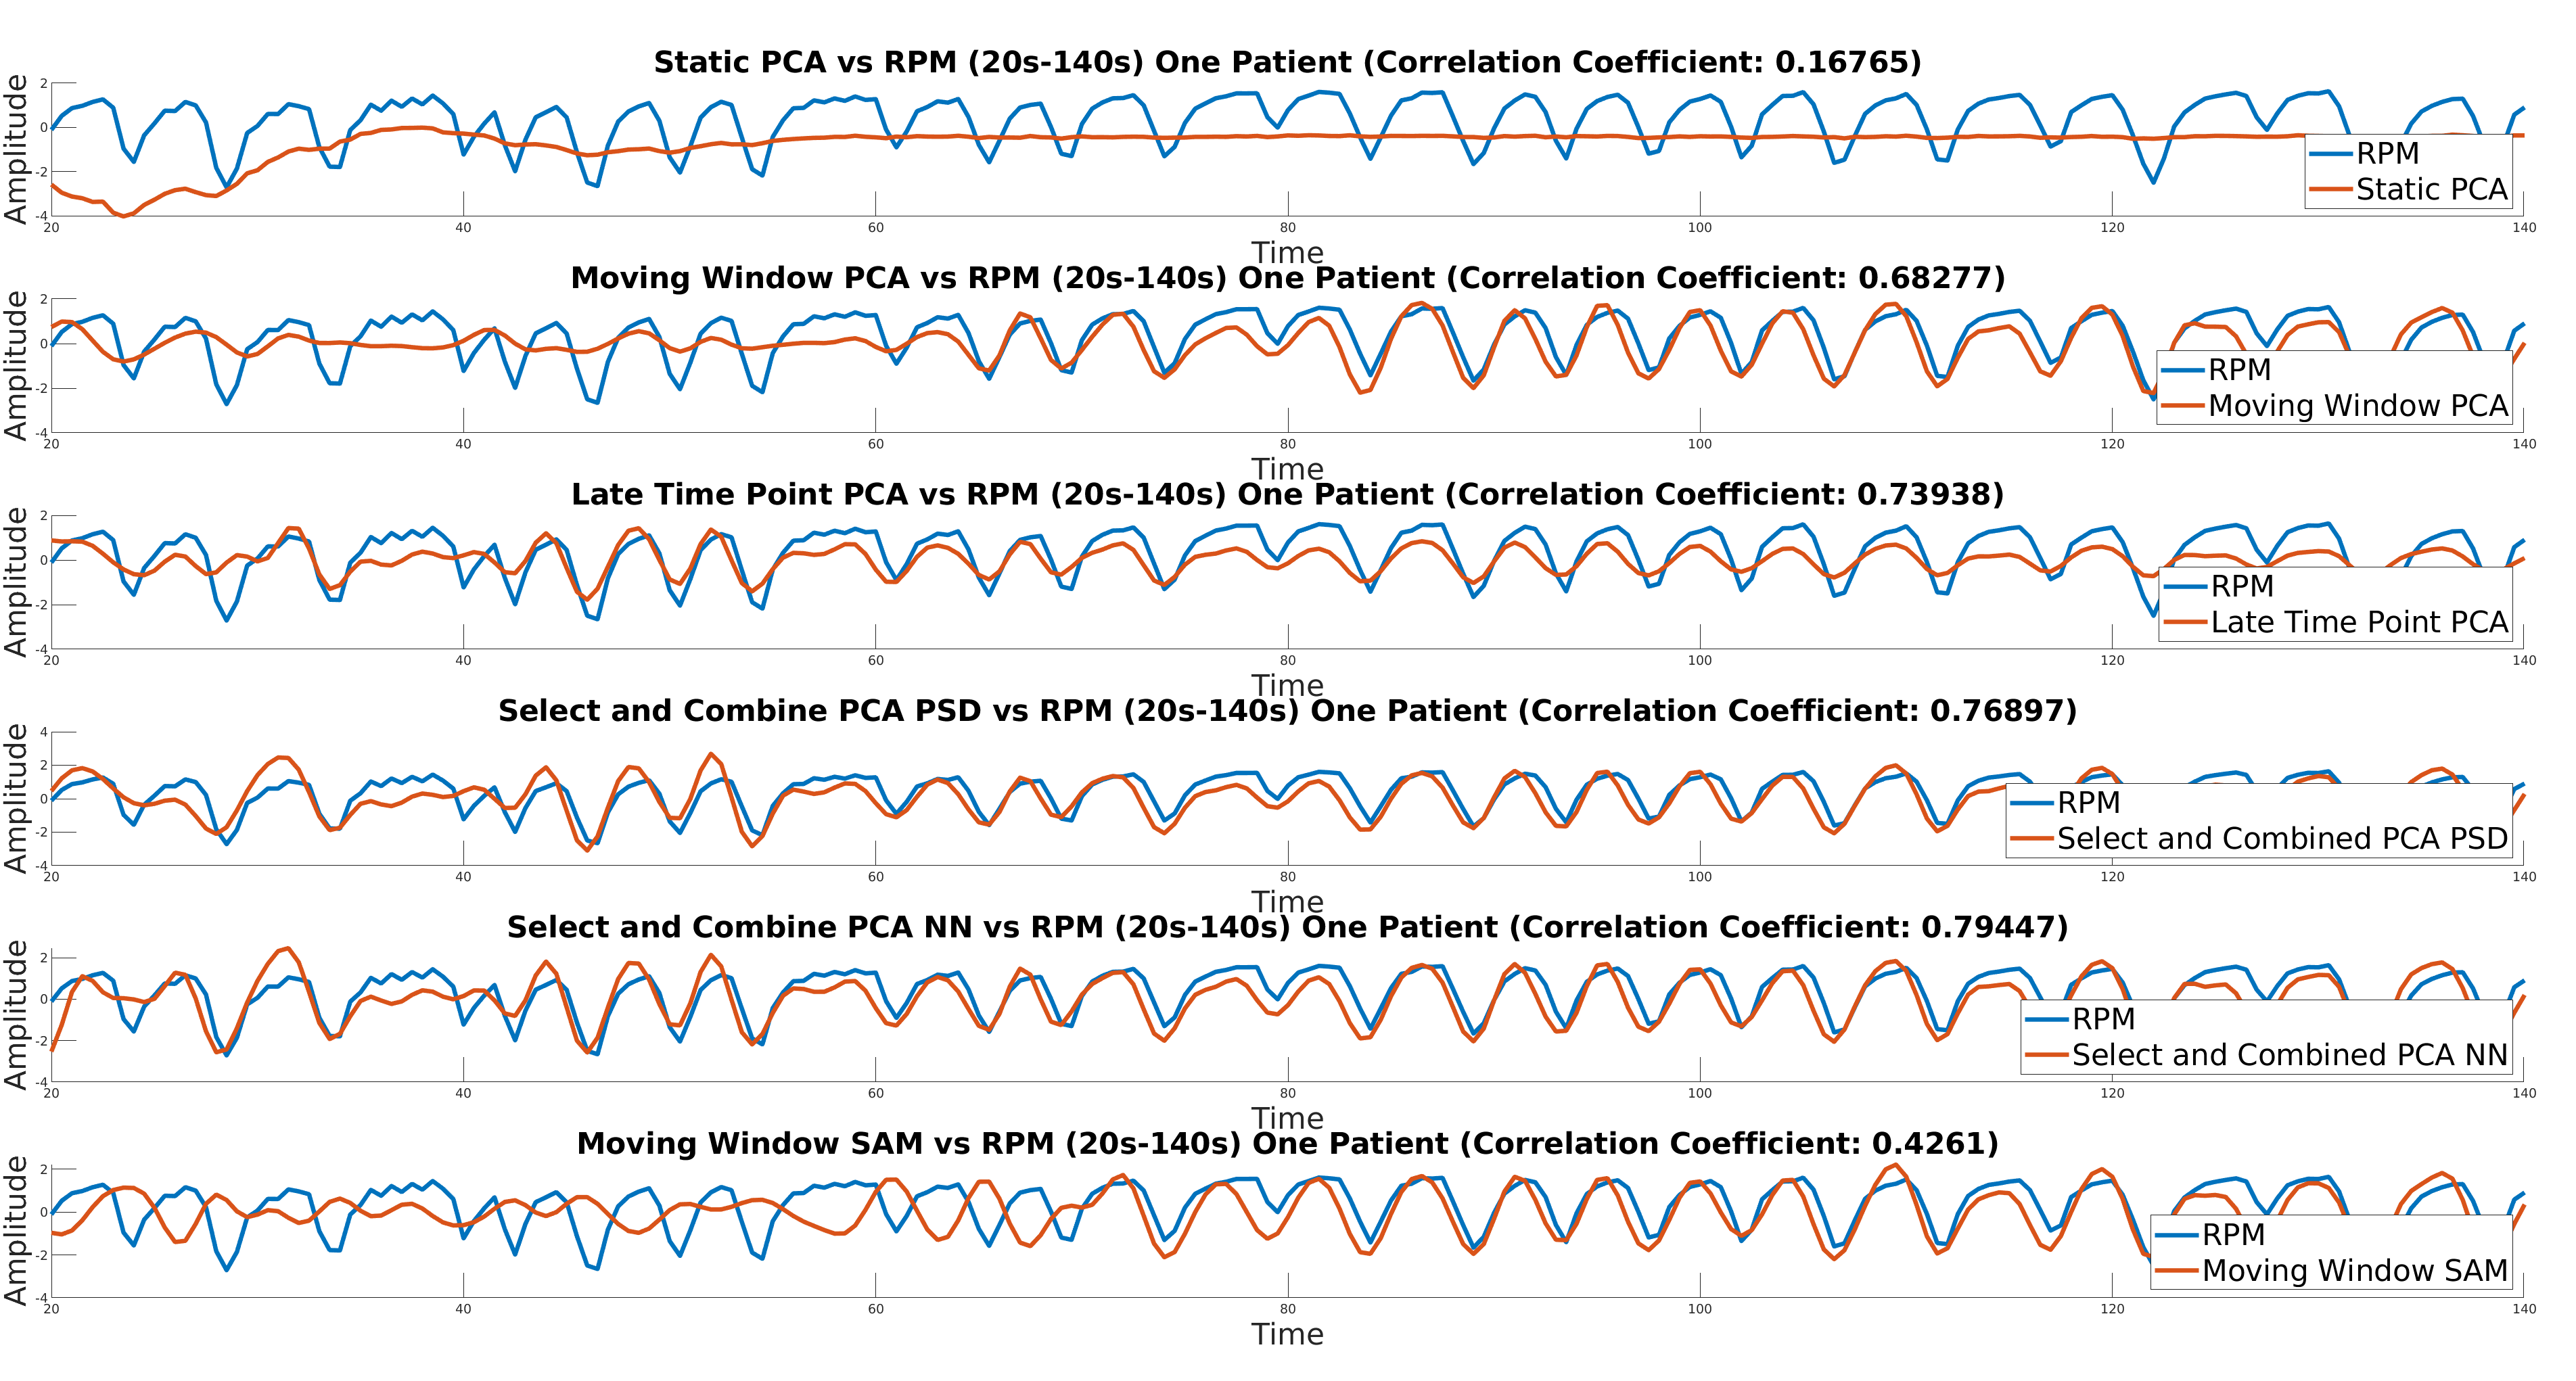
\includegraphics[width=0.9\linewidth]{figures/patient_one_output.png}
        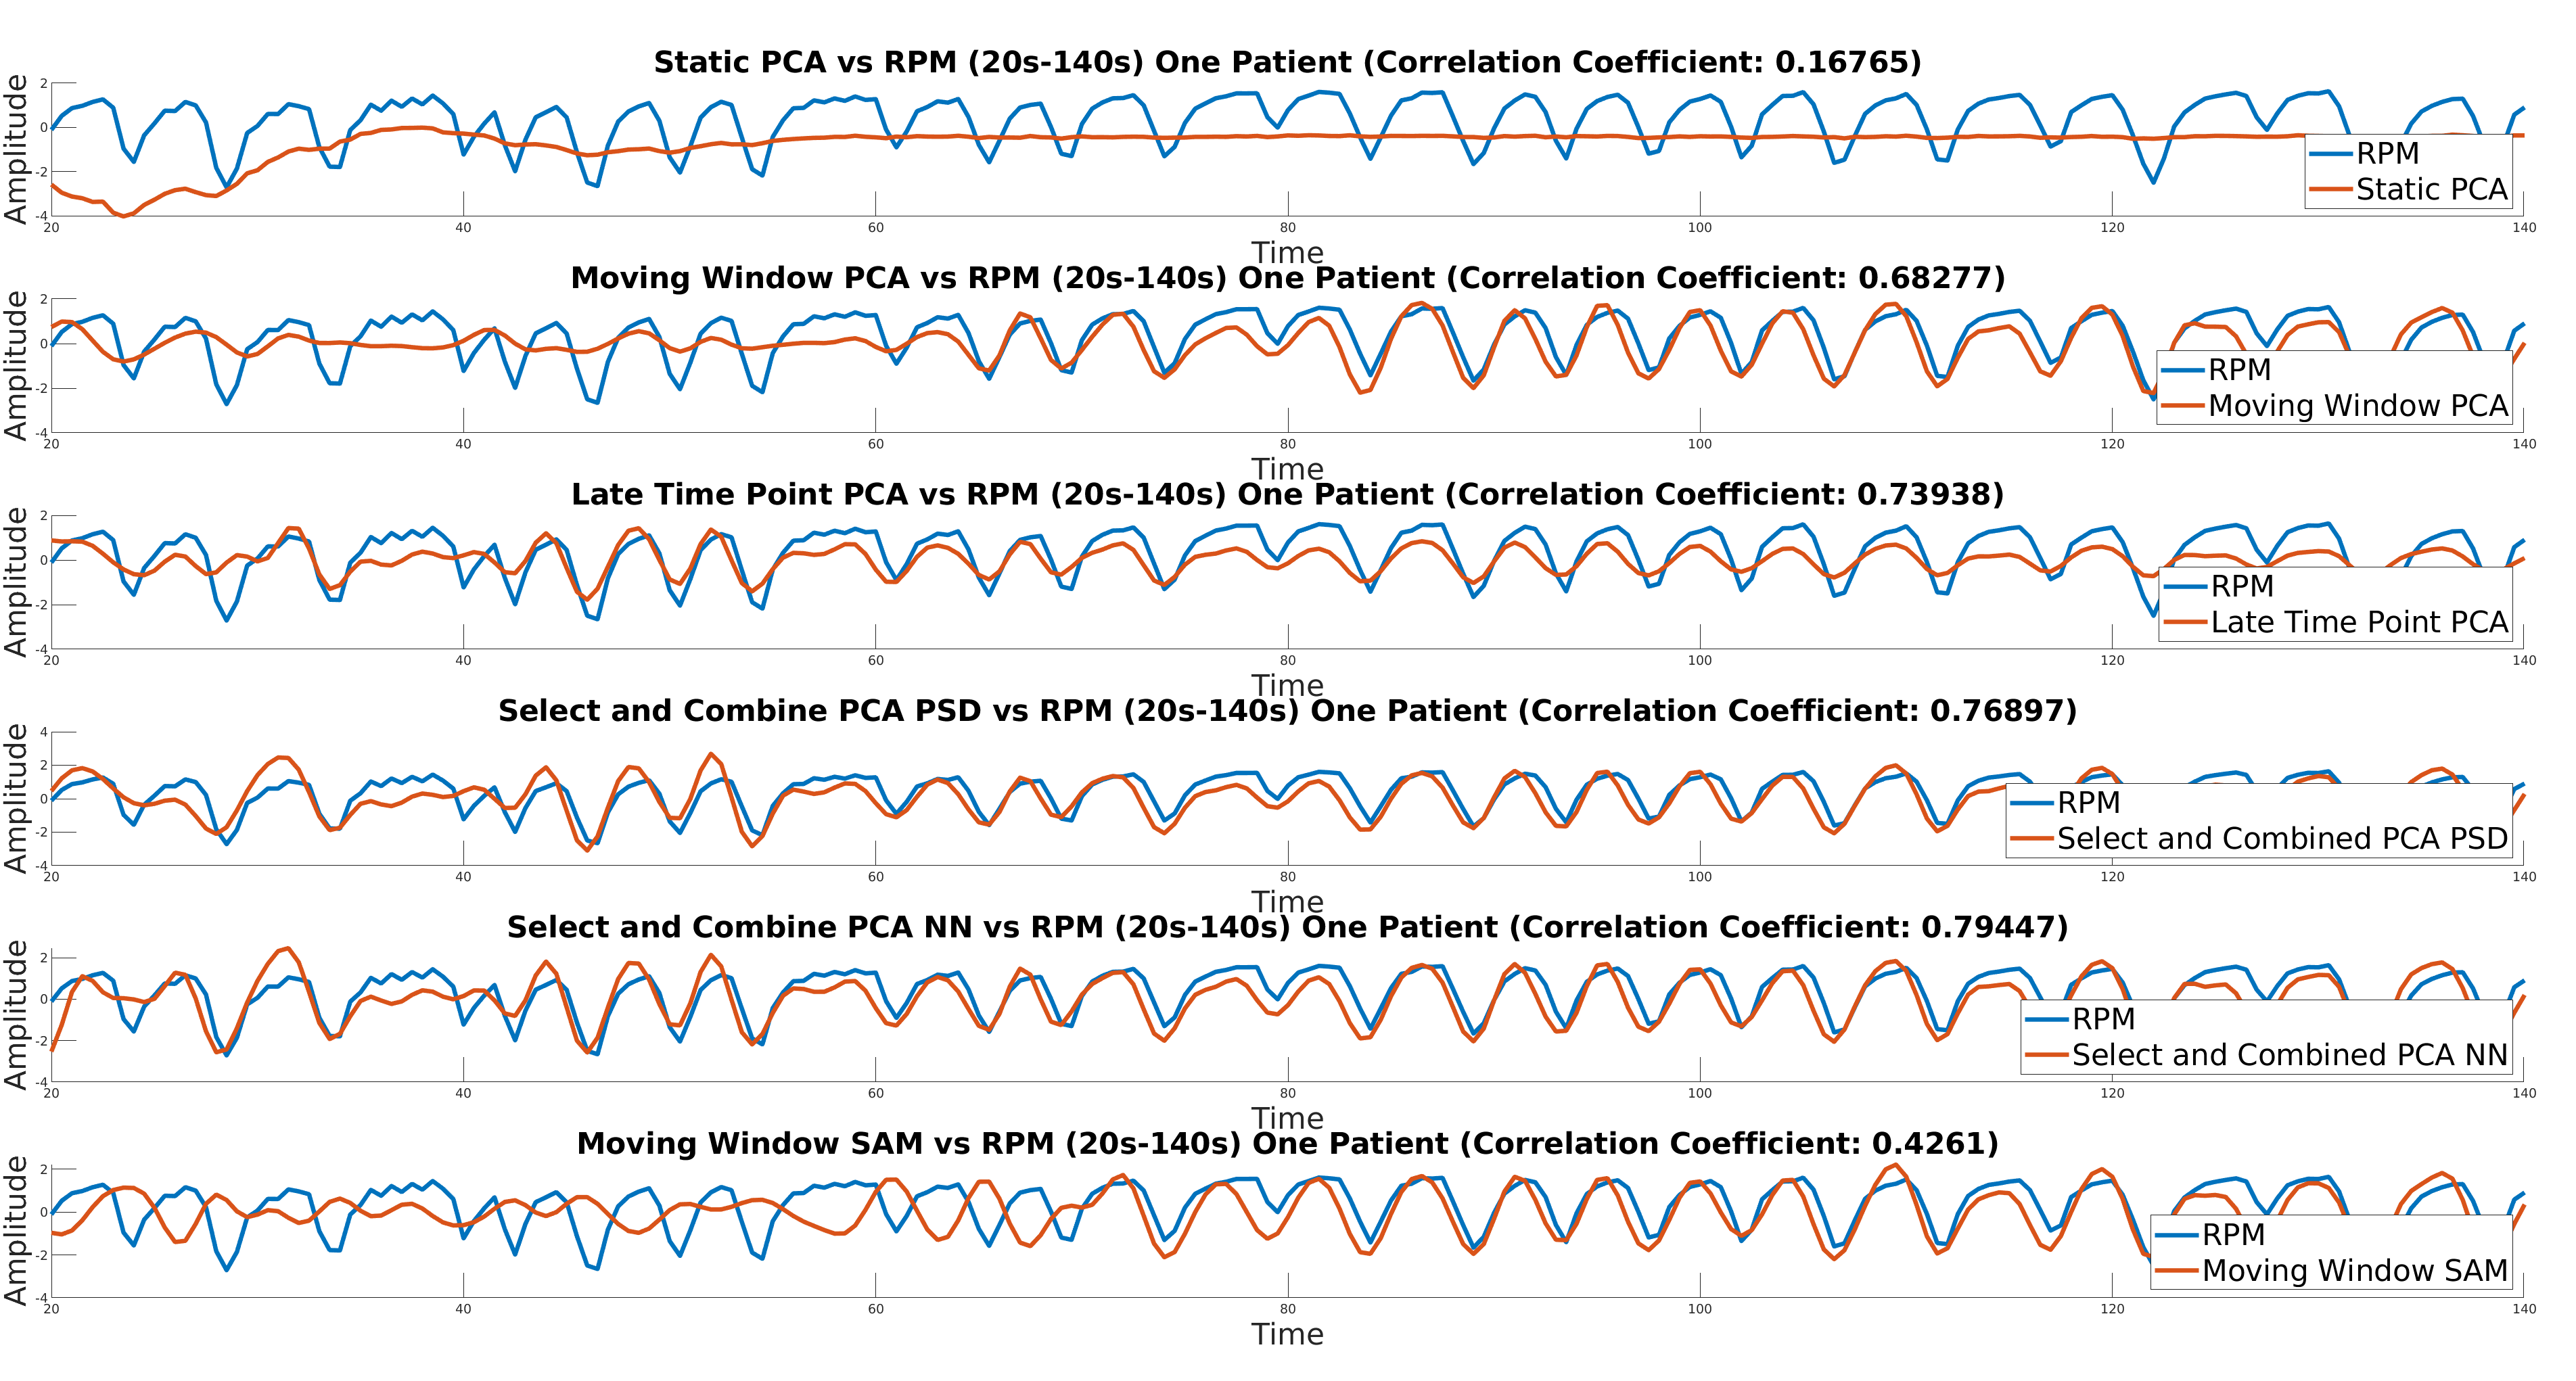
\includegraphics[width=1.0\linewidth]{figures/patient_one_output.png}
        
        \vspace{-0.4cm}
        
        \captionsetup{singlelinecheck=false, justification=centering}
        \caption{
        \scriptsize
        A plot showing for each method its output compared to the \gls{RPM} for the first \SI{120}{\second} (between \SI{20}{\second} and \SI{140}{\second}) (taken for the first acquisition of patient one).}
        
        \label{fig:patient_one_output}
        
        \vspace{-0.5cm}
    \end{figure}
    
    \begin{figure}
        \vspace{-0.5cm}
        
        \centering
        
        % 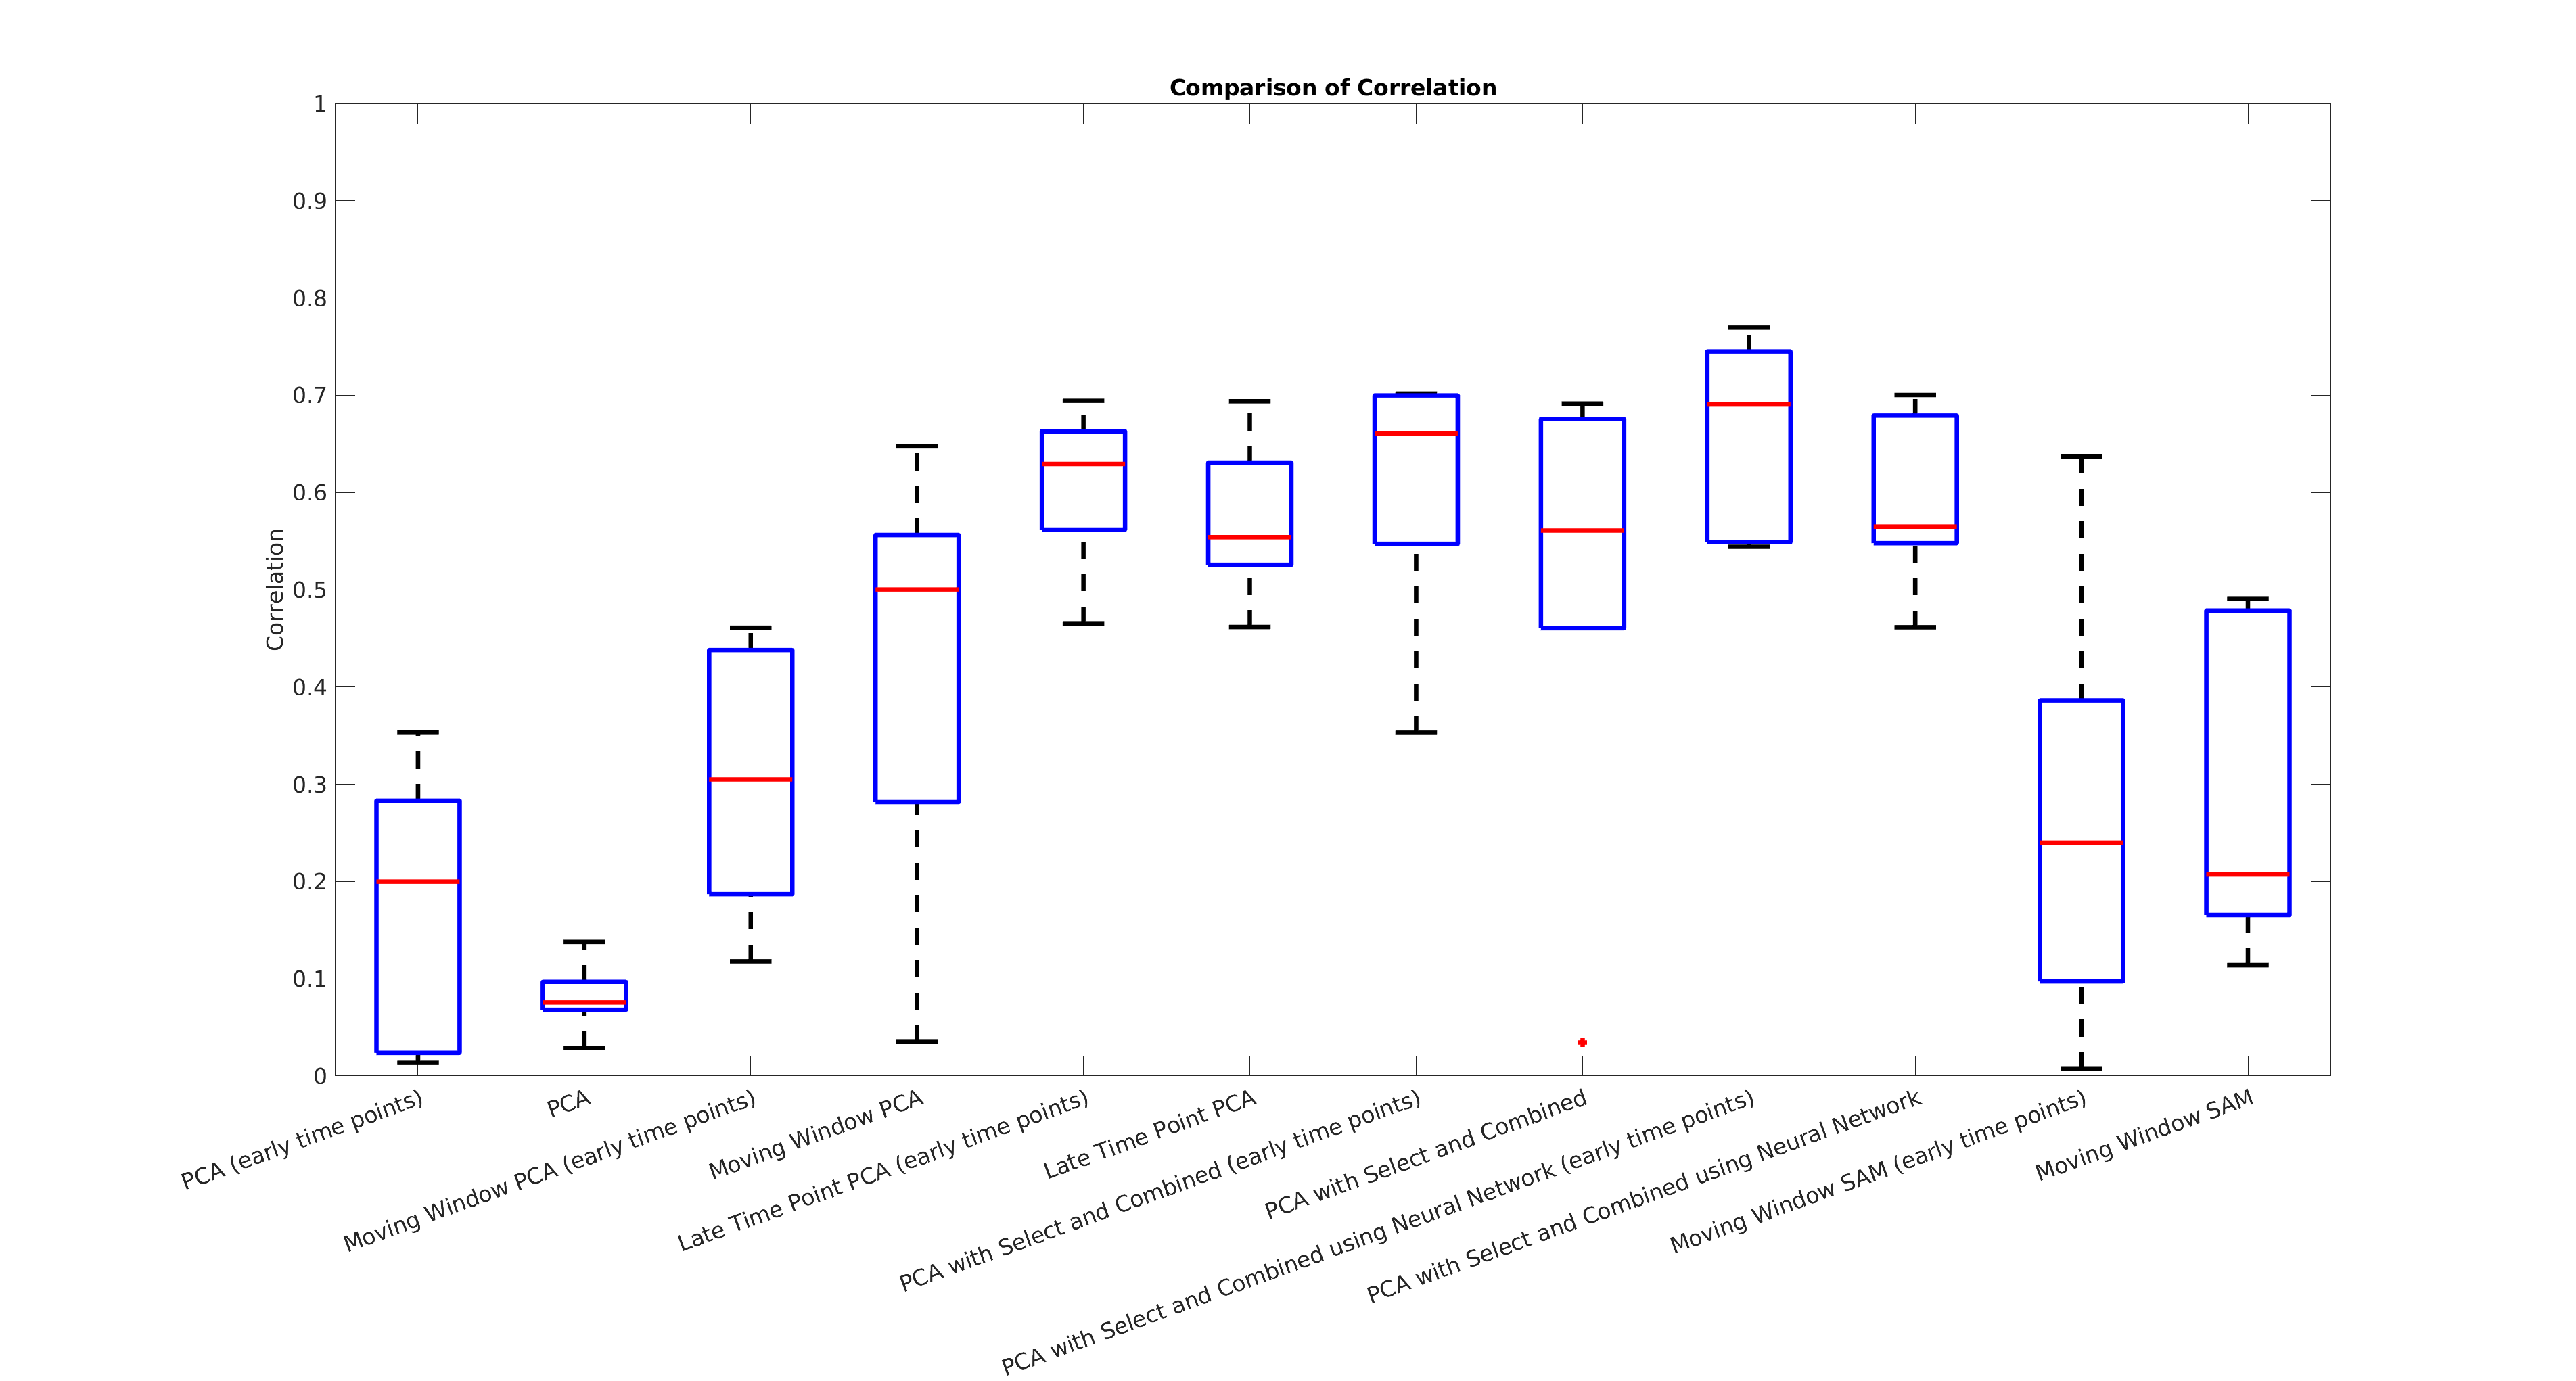
\includegraphics[width=0.9\linewidth]{figures/box_plot.png}
        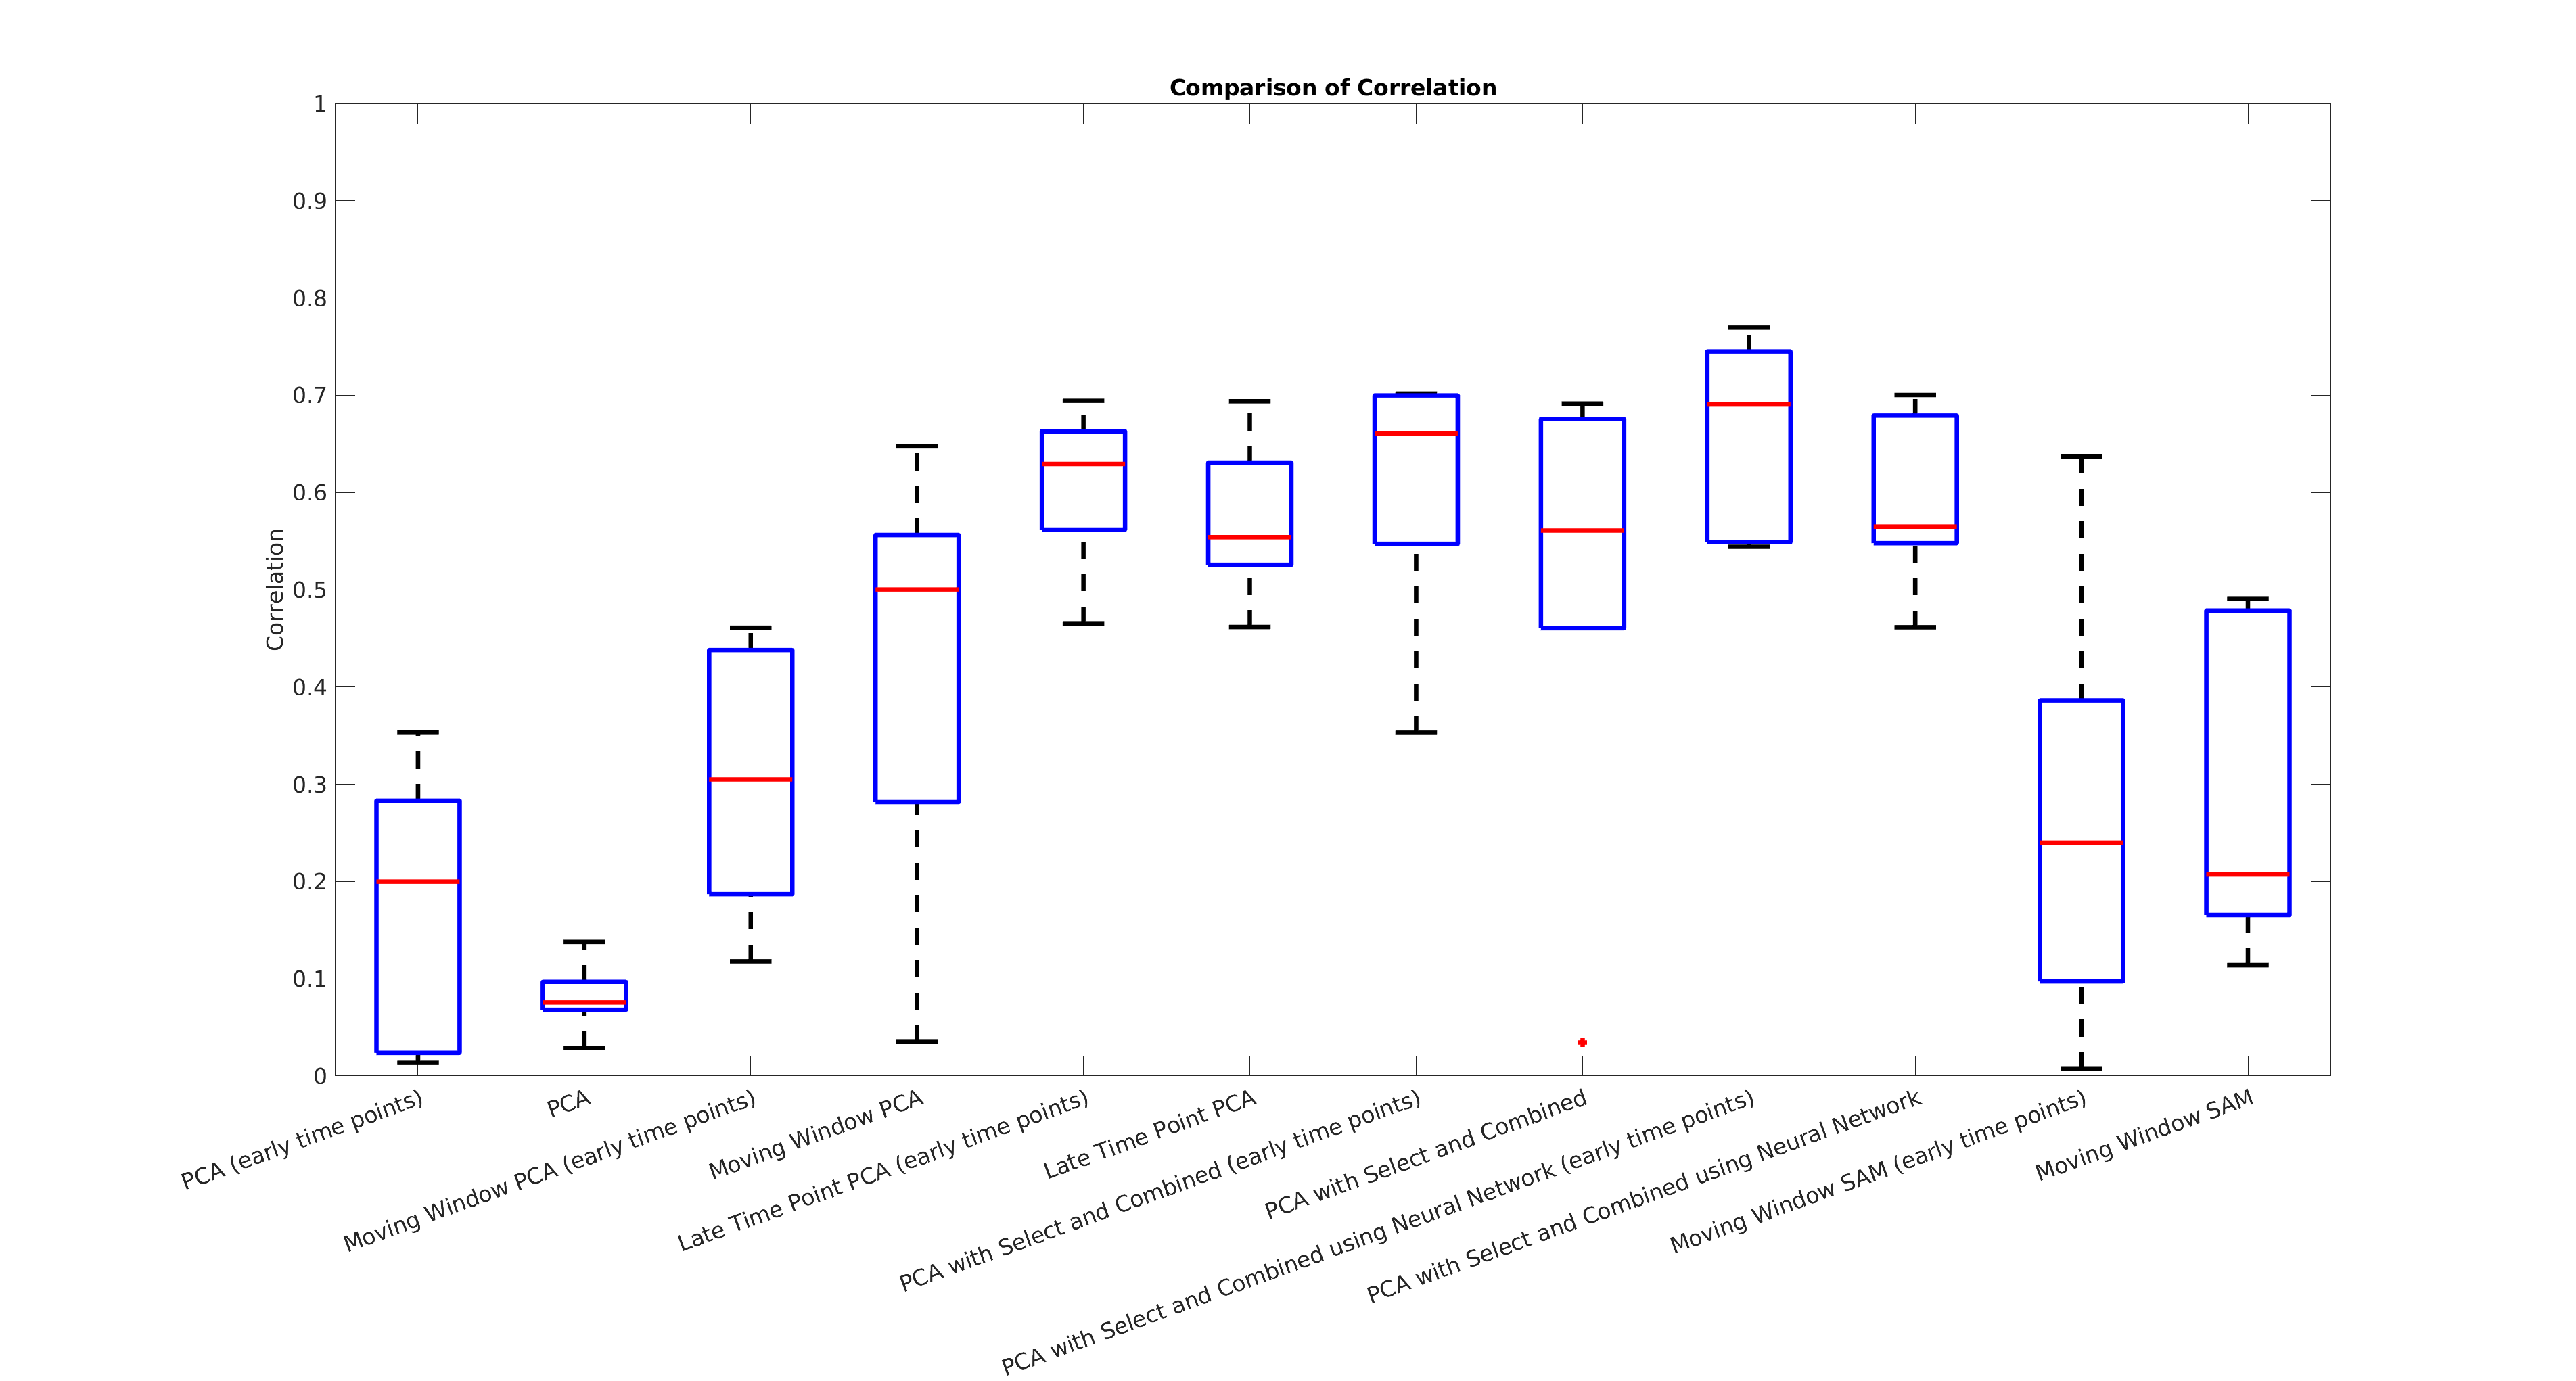
\includegraphics[width=1.0\linewidth]{figures/box_plot.png}
        
        \vspace{-0.4cm}
        
        \captionsetup{singlelinecheck=false, justification=centering}
        \caption{
        \scriptsize
        A box plot showing for each method its correlation coefficient to the \gls{RPM} for both the first \SI{120}{\second} (between \SI{20}{\second} and \SI{140}{\second}) and also for the entire acquisition (taken for seven acquisitions).}
        
        \label{fig:box_plot}
        
        % \vspace{-0.5cm}
    \end{figure}
    
    \begin{figure}
        % \vspace{-0.5cm}
        
        \centering
        
        % 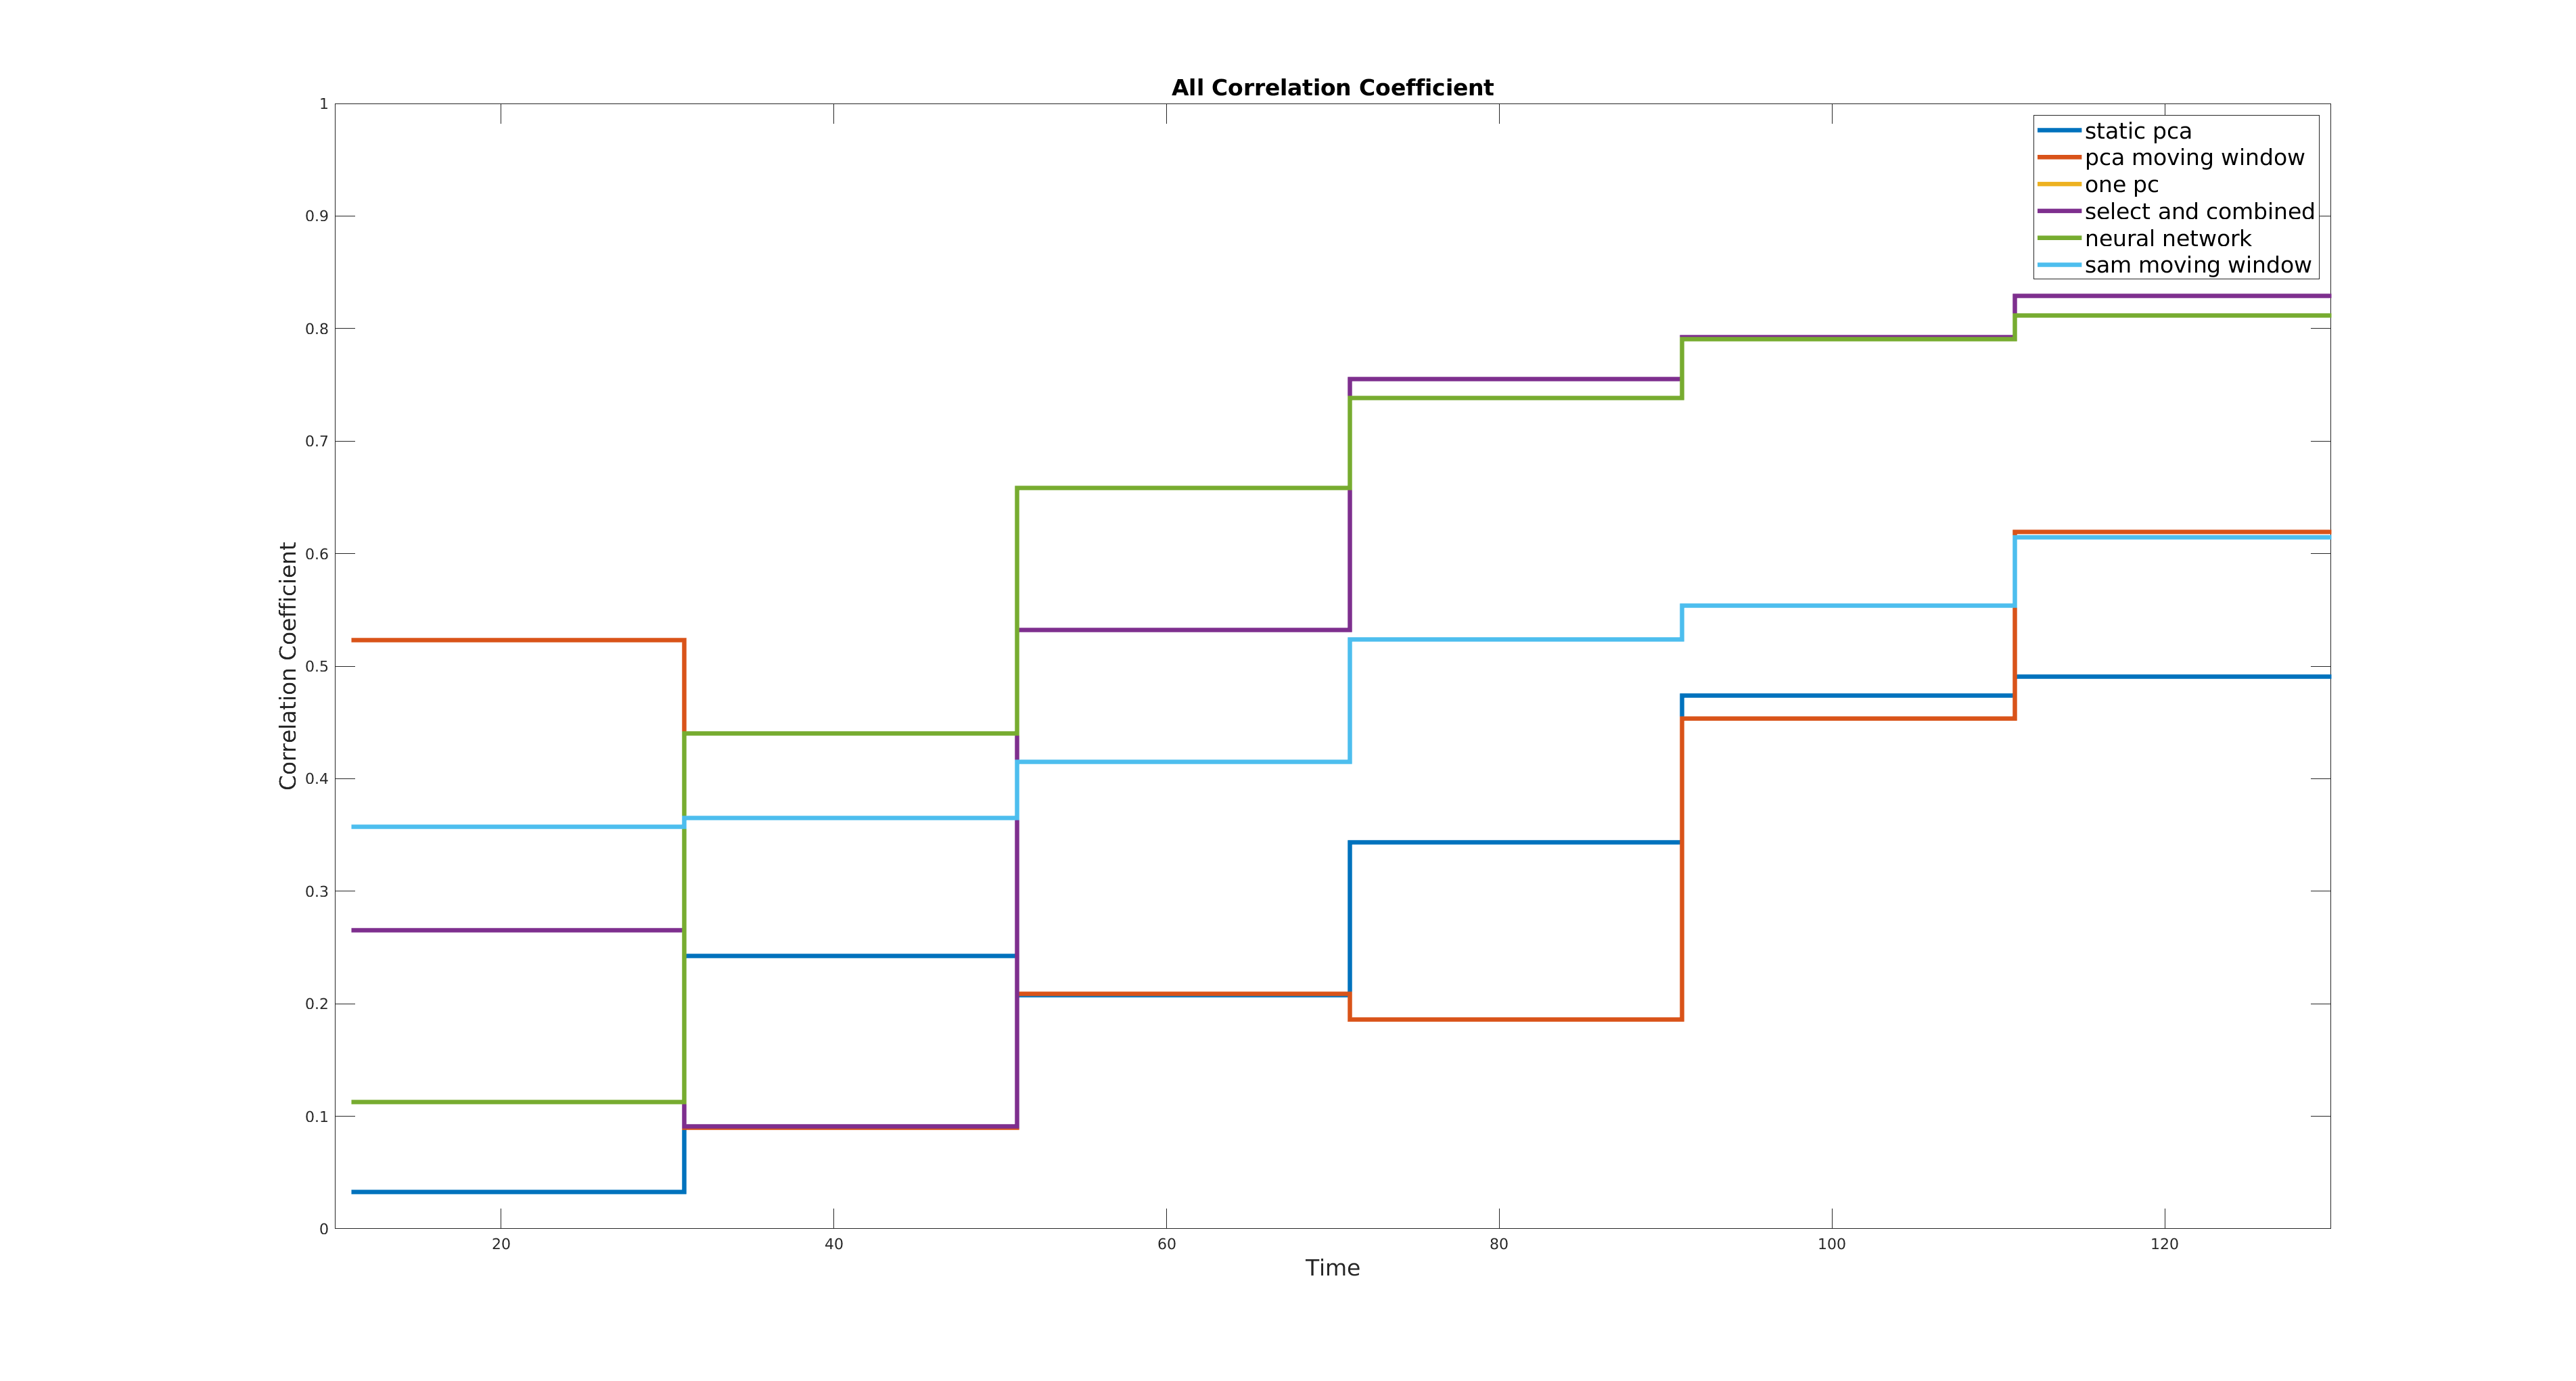
\includegraphics[width=0.9\linewidth]{figures/all_correlation_coefficient_stairs.png}
        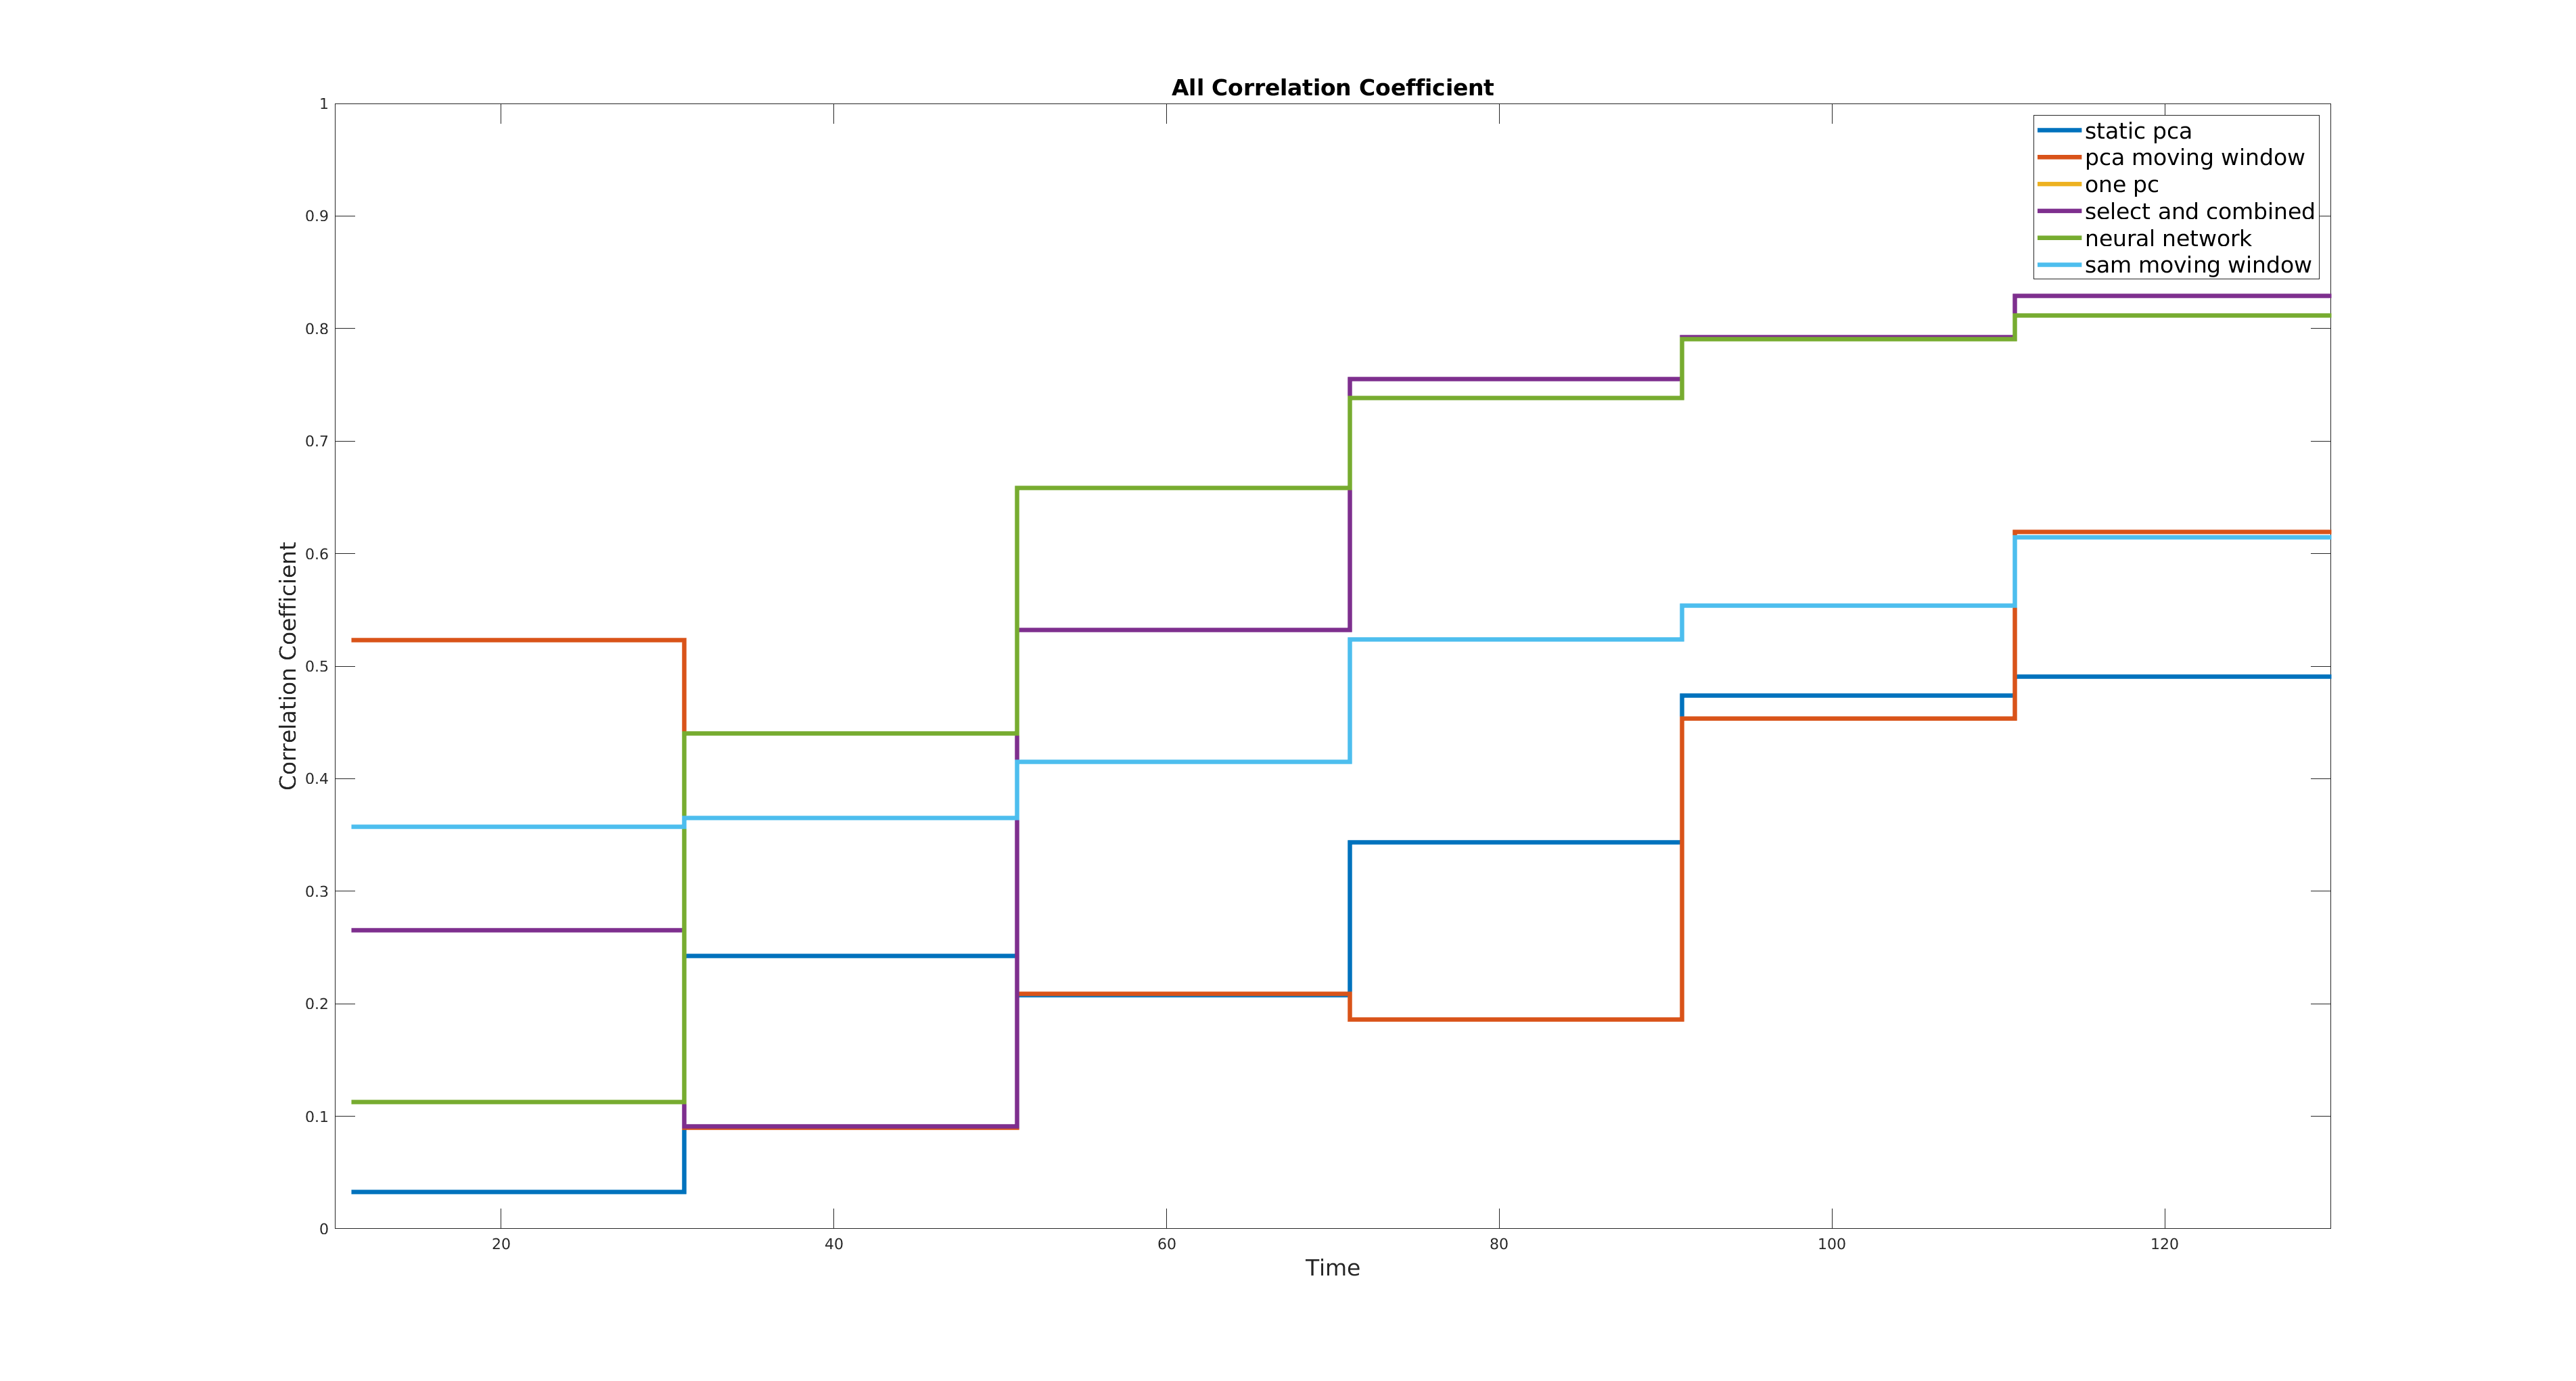
\includegraphics[width=1.0\linewidth]{figures/all_correlation_coefficient_stairs.png}
        
        % 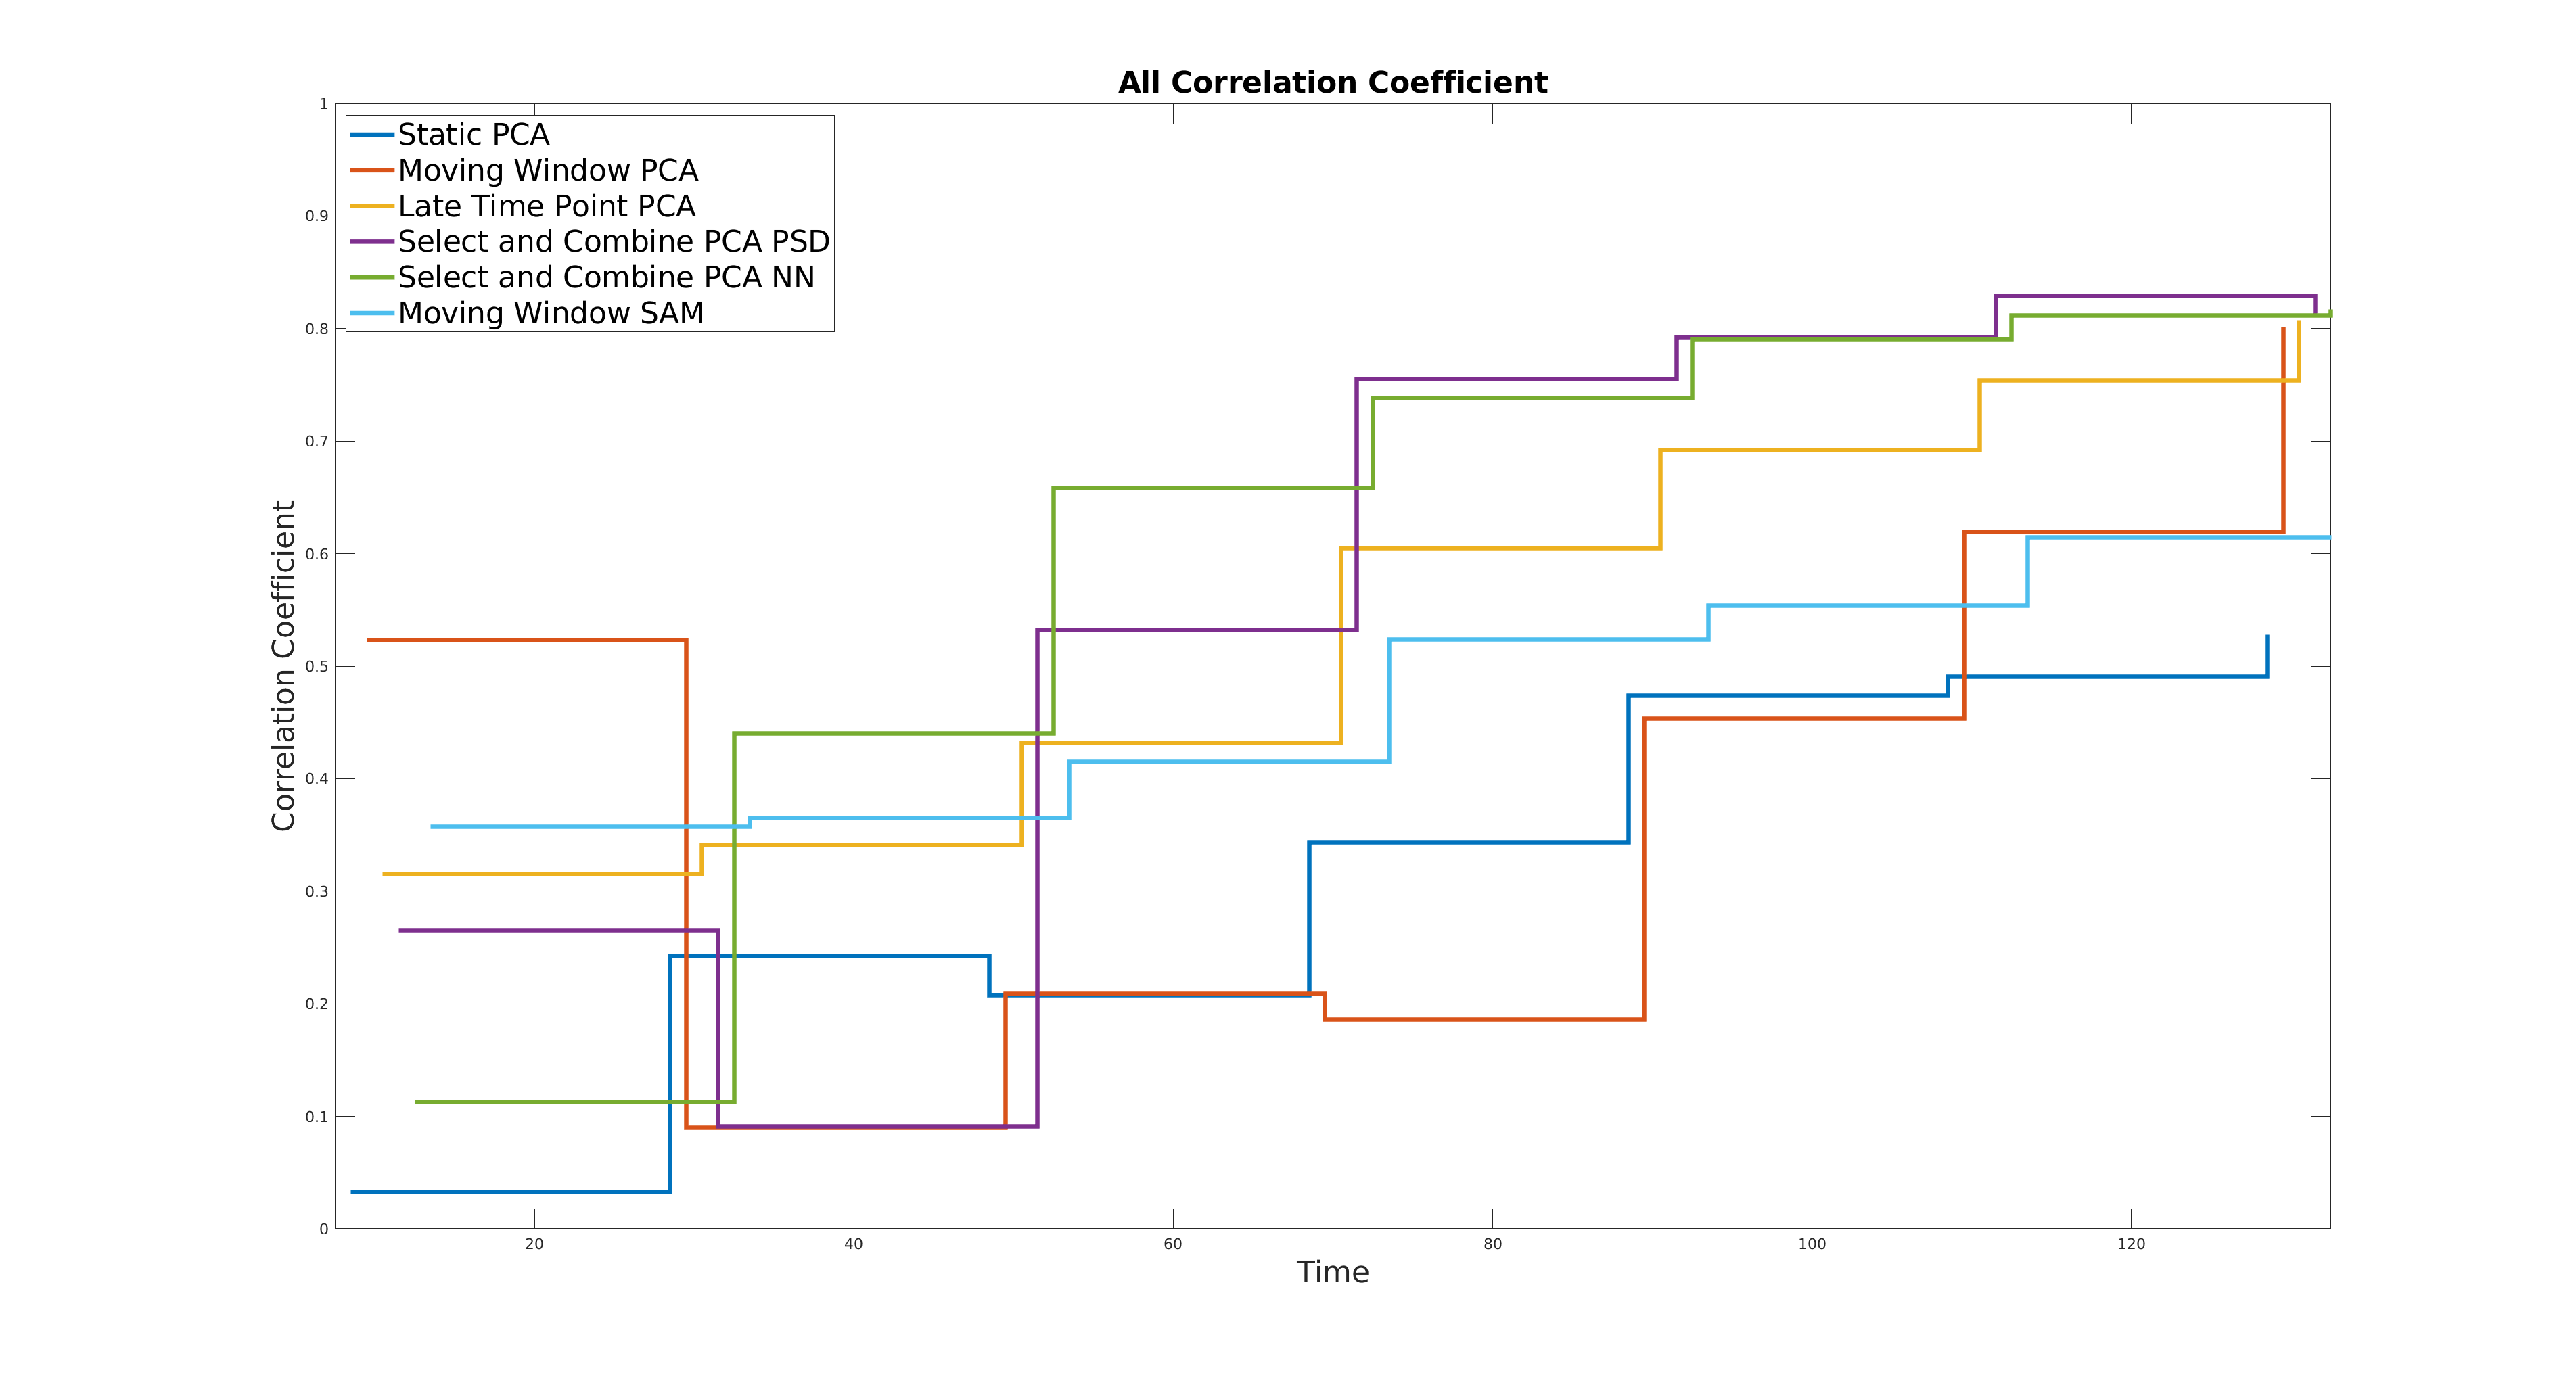
\includegraphics[width=0.9\linewidth]{figures/all_correlation_coefficient.png}
        % 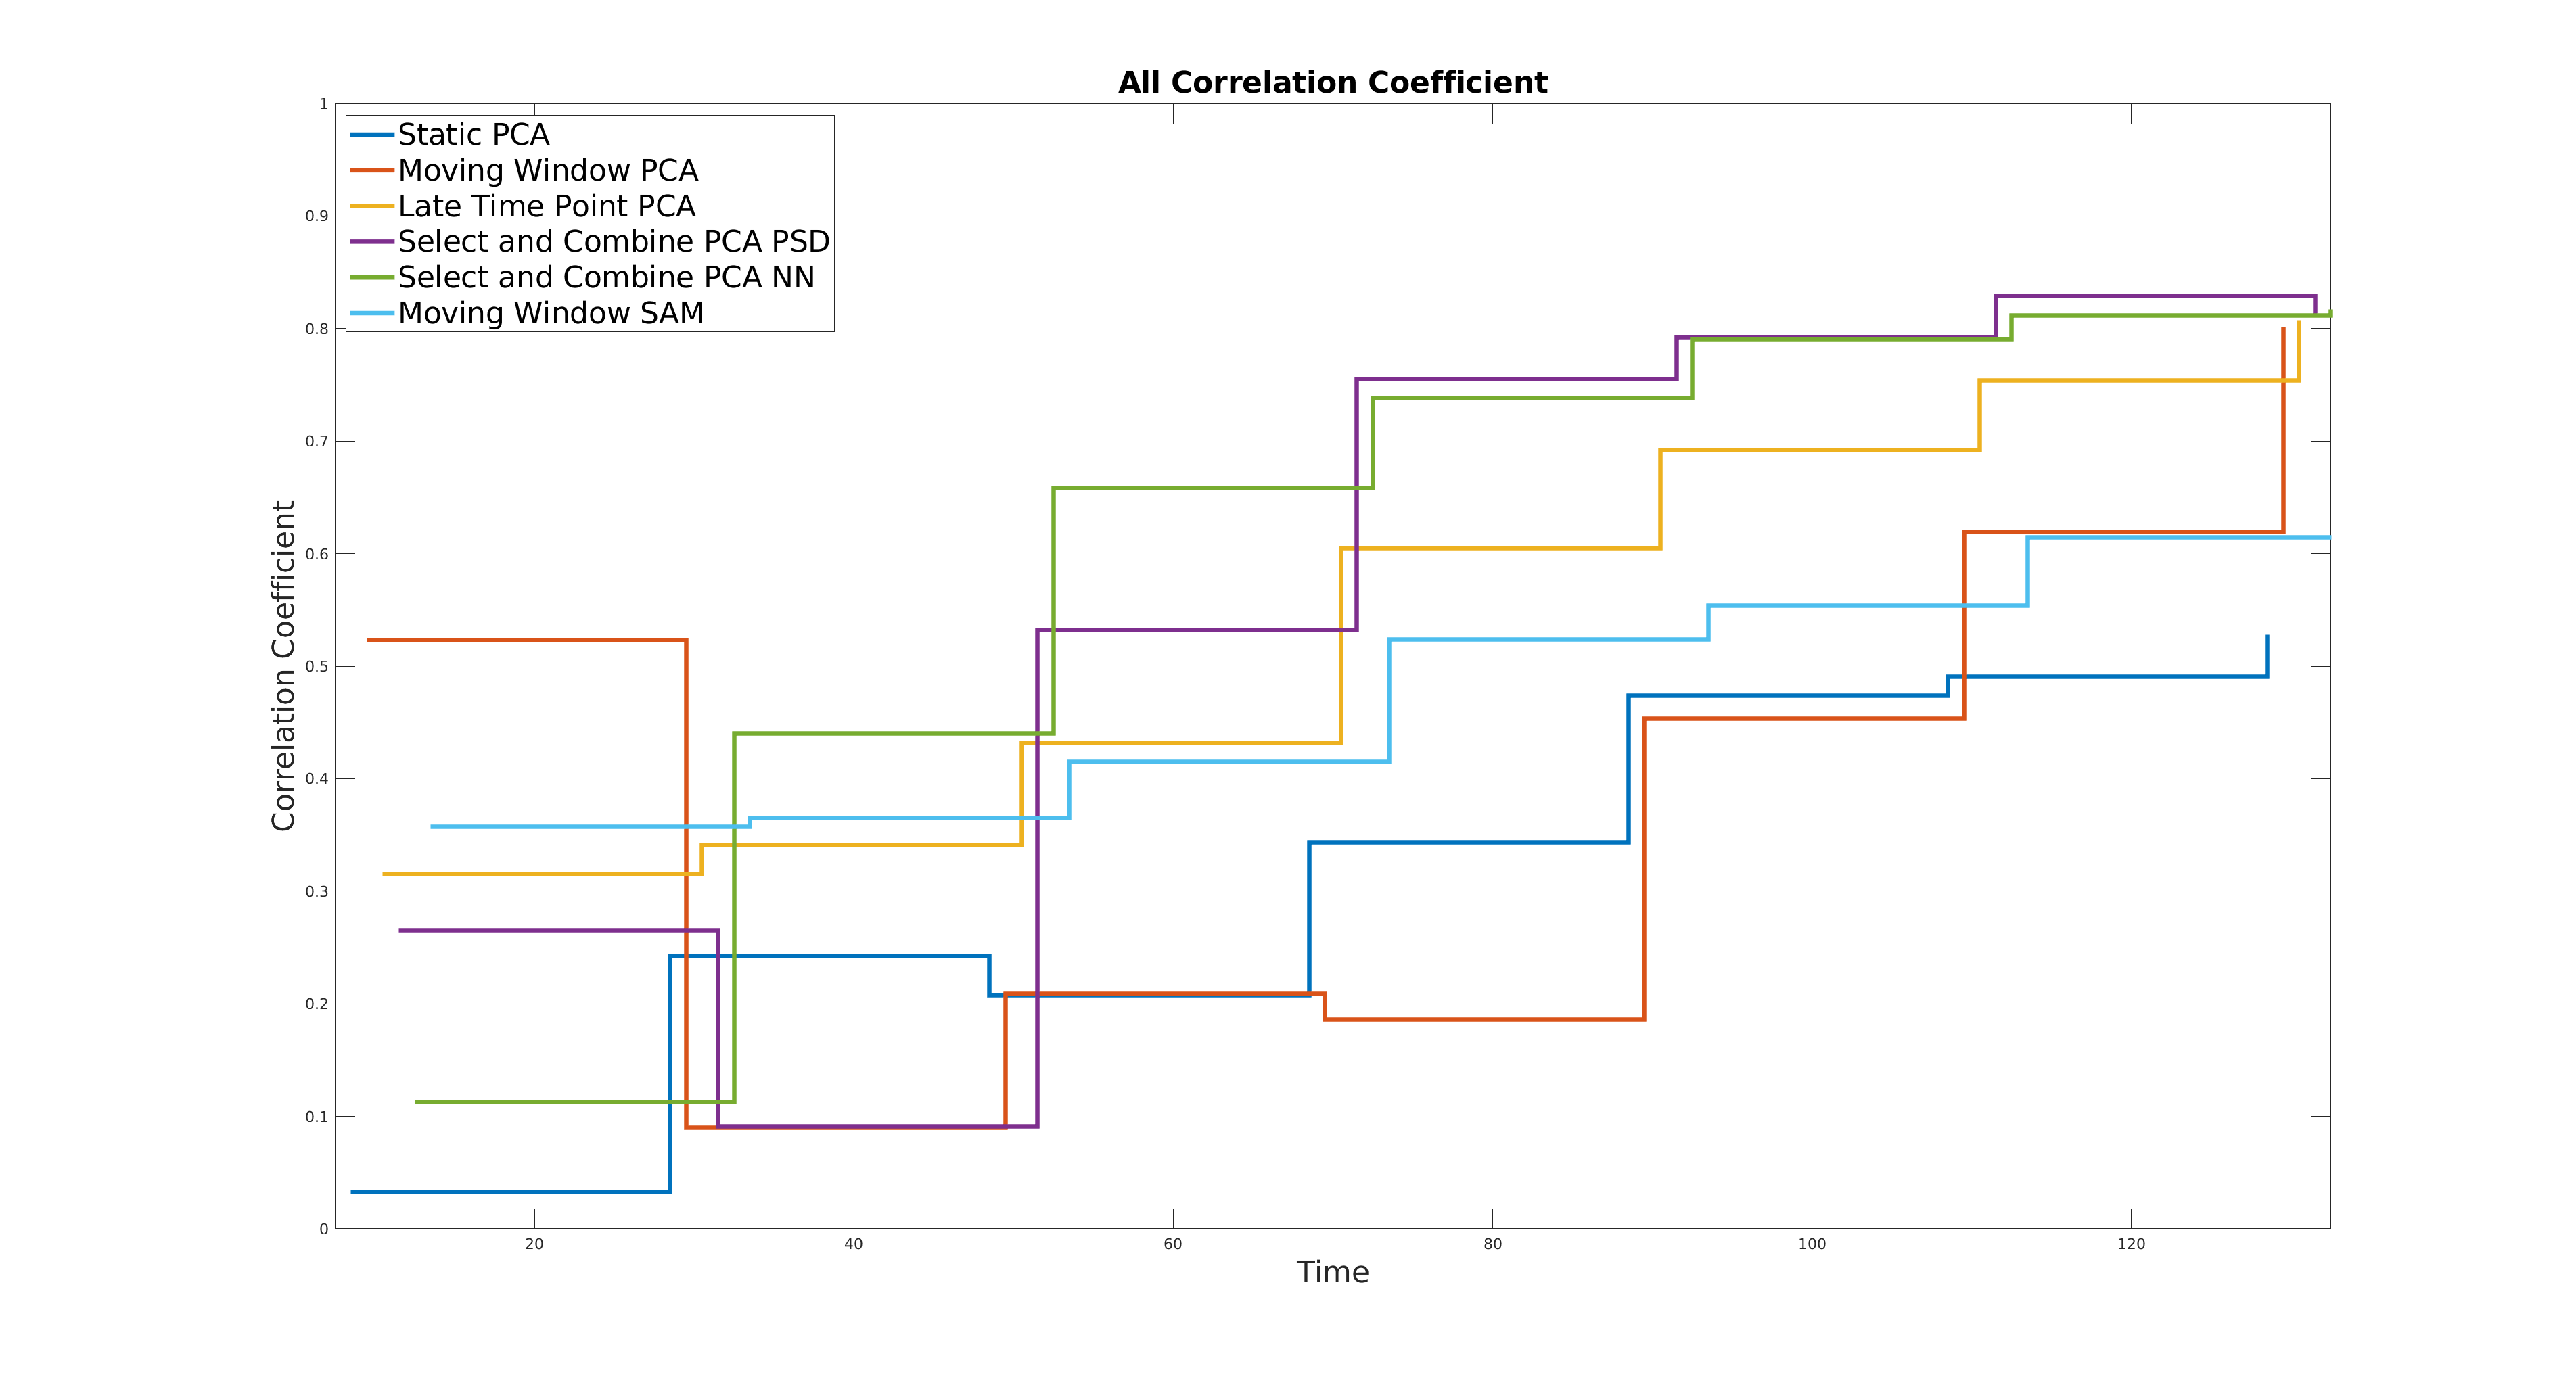
\includegraphics[width=1.0\linewidth]{figures/all_correlation_coefficient.png}
        
        \vspace{-0.5cm}
        
        \captionsetup{singlelinecheck=false, justification=centering}
        \caption{
        \scriptsize
        A plot showing for each method its correlation coefficient to the \gls{RPM} for the first \SI{120}{\second} (between \SI{10}{\second} and \SI{130}{\second}, in twenty second windows) (taken as a mean for all data).}
        
        \label{fig:all_cross_correlation}
        
        \vspace{-0.5cm}
    \end{figure}
    
    % \begin{figure}
    %     \vspace{-0.5cm}
    %     \centering
    
    %     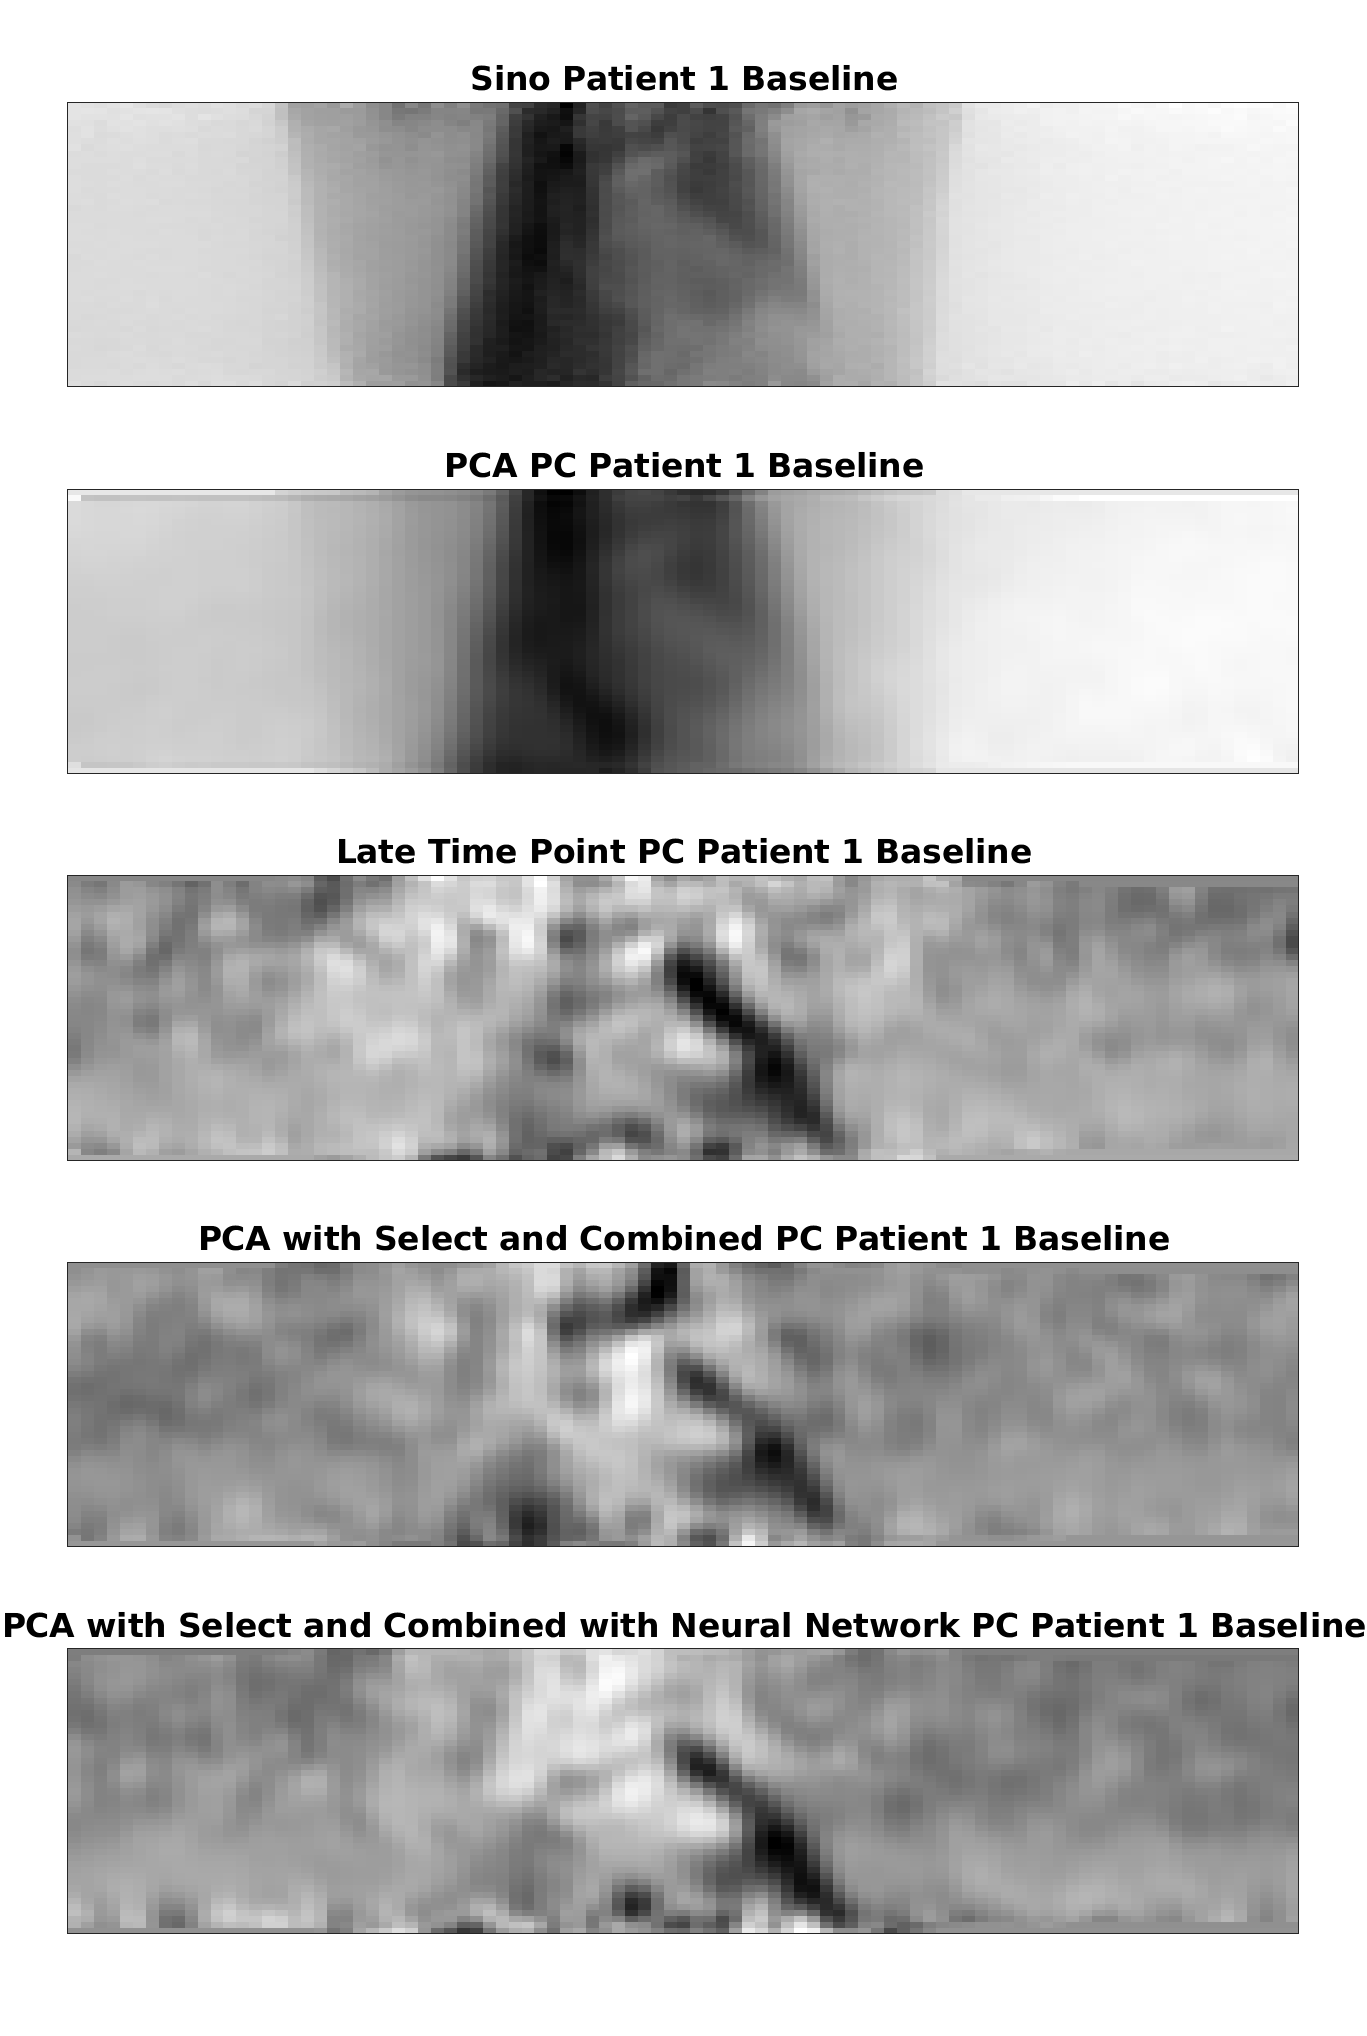
\includegraphics[width=1.0\linewidth]{figures/patient_one_pc_output.png}    
    %     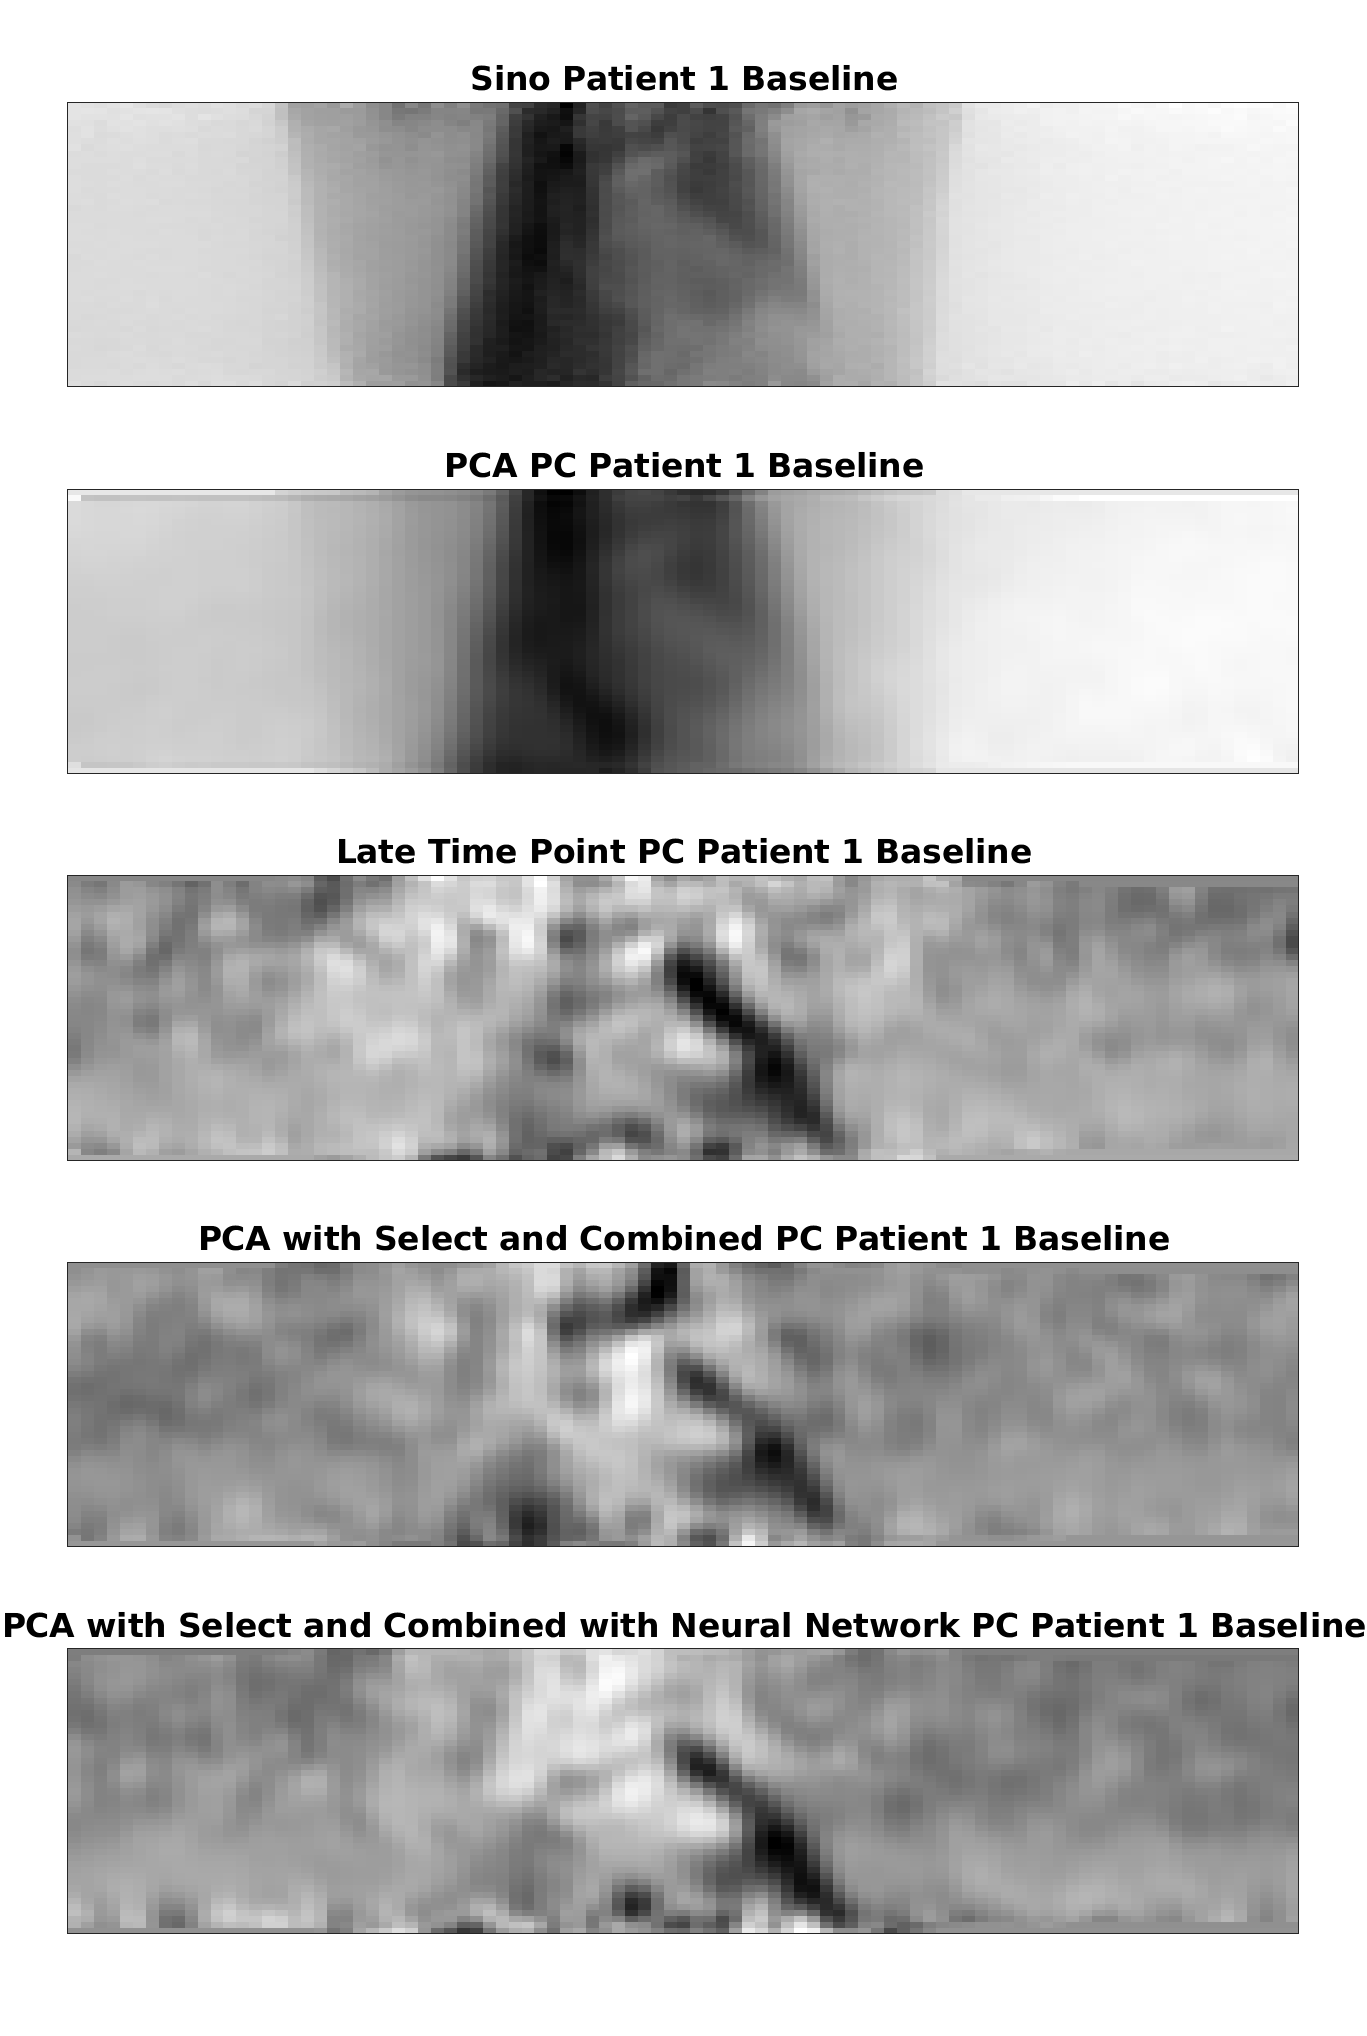
\includegraphics[width=1.0\linewidth]{figures/patient_one_pc_output.png}
    
    %     \vspace{-0.5cm}
        
    %     \captionsetup{singlelinecheck=false, justification=centering}
    %     \caption{
    %     \scriptsize
    %     A plot showing the \gls{PC} used to generate the output signal (taken for the first acquisition of patient one).}
    
    %     \label{fig:patient_one_pc_output}
    
    %     \vspace{-0.5cm}
    % \end{figure}
    
     From~\Fref{fig:patient_one_output} and~\Fref{fig:all_cross_correlation} it can be observed that the static \gls{PCA} method has failed as expected. Both moving window methods extract a signal at later time points only.. The Late Time Frame \gls{PC}, Select and Combine and Select and Combine using a Neural Network methods all appear to be able to extract a usable signal down to \SI{20}{\second} after the start of the scan.
    
    In~\Fref{fig:box_plot} the improvement of the Late Time Frame \gls{PC} and by incorporating multiple \glss{PC} is most apparent with high correlation coefficient for both the early time point as well as for all data. The Select and Combine methods show marginally higher correlation coefficient than the Late Time Frame \gls{PC} method and the neural network shows slightly higher correlation coefficient than the frequency based scoring.
    
    % In~\Fref{fig:patient_one_pc_output} it can be observed the static \gls{PCA} method returns a \gls{PC} which closely resembles the input data, leading to the conclusion that variation from a number of sources is included. It appears from a visual inspection that the least confounding variation and noise is included in the Select and Combine with Neural Network method.

\vspace{-0.5cm}

\section{Discussion and Conclusions} \label{sec:discussion_and_conclusions}
    Results from the comparison to the \gls{RPM} indicate that the Late Time Frame \gls{PC} and both Select and Combine methods are more robust and afford higher quality signals than both moving window methods. The results also indicate that both Select and Combine methods can give a higher correlation coefficient earlier than the Late Time Frame \gls{PC} method and that the neural network shows slightly higher correlation coefficient than the frequency based scoring.
    
    In the future, research will focus on further development of the method, including optimisation of the neural network scoring method. In the next stage, these methods will be applied to the task of implementing advanced respiratory motion correction on dynamic \acrshort{PET} data.